Although McG paper does not clearly state any results of the agents individually, this thesis aims to investigate the integrity of the implementation. This will be done by examining the agents' algorithm in detail , along with the specific parameters in addition to looking at cited papers in McG which relates to where the McG's agents are based from. The aim of this section is to ensure that if the system (the new BSE) and the agents themselves are performing like what they are meant to do, we can be certain that any experiment results from the market consisting of the 5 agents will be valid. 


\section{Market maker}
The Market maker in McG is modelled closely to Oesch 2014 conference paper \cite{Oesch}. 

\begin{table}[h]
\centering
\begin{tabular}{ |m||p{4cm}|} 
\hline
\textbf{Market maker Parameters}& \textbf{Value} \\
\hline
\hline
$v_{min}$ & 100 \\ 
\hline
$v_{max}$ & 200,000\\ 
\hline
$v^-$ & 1\\ 
\hline
$w$ & 50\\
\hline
\end{tabular}
\caption{Market maker trader parameters taken from \cite{McGroarty} and  \cite{Oesch}} 
\end{table}
\FloatBarrier 

To clarify, the Market maker will make its decision based on a moving average of $w$ period. The moving average is calculated from the number of bids and asks in the $w$ period. In McG, the paper refers to Long Term memory order flow such that the future order is heavily correlated with the orders in the past. In each period, a buy order is given a +1 and a sell -1. The sum of those, if is positive, the Market maker agent will submit an ask large order with best price and quantity uniformly distributed from $U(v_{min},v_{max})$ and a bid order with quantity = $v^-$. Vice versa, if the sum of the period is negative. 

In order to test the Market maker behaviour, two simpler agents is implemented called Simple Buyer and Simple Seller. The Simple Buyer and Seller will only submit a bid or an ask order with price = $100$ in any circumstances with quantity uniformly distributed between 1 and 100. The total time period is 100 running with McG time system. A short experiment is conducted where a market consisting of 6 Market makers and 6 of one of the Simple agents. The expected behaviour is that the Market maker will submit only an Ask order in a market with Simple Buyer since it will try to match the incoming bid orders. Vice versa for a market with Simple Seller. 

\begin{figure}[h]
  \begin{subfigure}[b]{0.5\textwidth}
    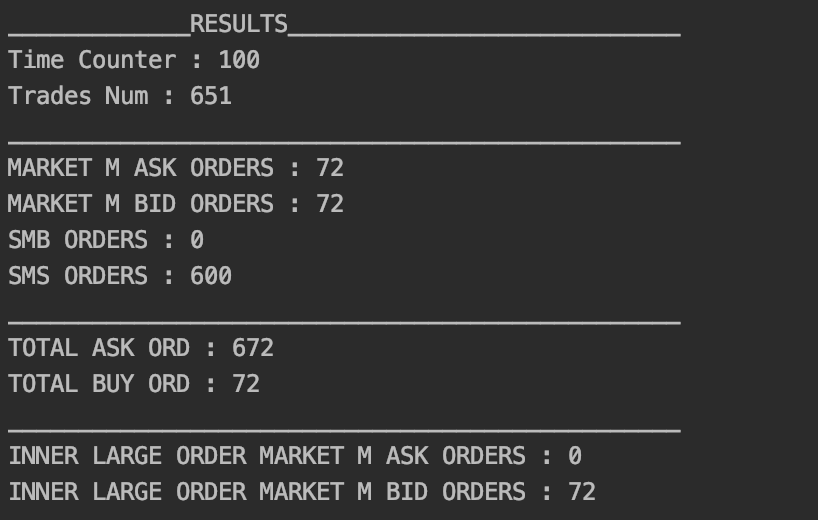
\includegraphics[width=7cm, height=6cm]{Dissertation/images/mcg_indv/SMS.png}
    \caption{Market maker with Simple Seller}
    \label{fig:1}
  \end{subfigure}
  %
  \begin{subfigure}[b]{0.5\textwidth}
    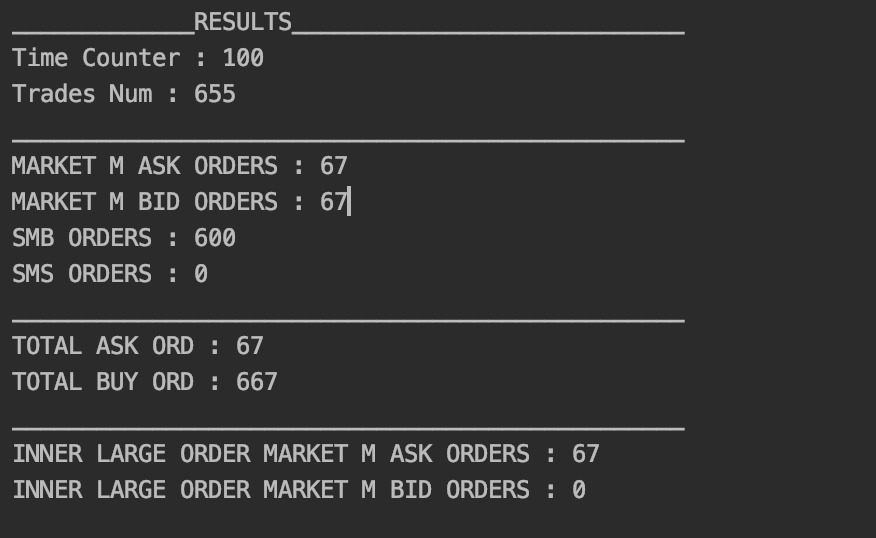
\includegraphics[width= 7cm, height=6cm]{Dissertation/images/mcg_indv/SMB.png}
    \caption{Market maker with Simple Buyer}
    \label{fig:2}
  \end{subfigure}
\caption{Market maker with Simple agent statistics} 
\end{figure}

In figure 5.1(a), it can be seen that the bid large order of the Market maker is the only one submitted (72 submitted). This is because all of the orders in the Market submitted by the Simple Seller is an ask order. In addition, the number of total asks and bids submitted by the Market maker is also 72 because in each iteration, the Market maker submits both a bid and an ask order with the bid order at quantity $v^-$. Vice versa with figure 5.1(b) where only ask large orders are submitted. 

\section{Liquidity consumer} 
In McG, the Liquidity consumer is also modelled closely to the Oesch 2014 \cite{Oesch} paper. The only difference is that in Oesch's paper, the Liquidity consumer will trade according to a large order, if empty, will generate a new one. However, in the McG paper, if the initial large order at the start of the day is empty, the Liquidity consumer will stop trading. 
\begin{table}[h]
\centering
\begin{tabular}{ |m||p{4cm}|} 
\hline
\textbf{Liquidity consumer Parameters}& \textbf{Value} \\
\hline
\hline
$h_{min}$ & 1 \\ 
\hline
$h_{max}$ & 100,000\\ 
\hline
\end{tabular}
\caption{Liquidity consumer parameters taken from \cite{McGroarty} and  \cite{Oesch}} 
\end{table}
\FloatBarrier 

Because the Liquidity consumer only submits a market order, the only test that is viable is to see its quantity submitted. There are two cases that the quantity of a Liquidity trader will differ. The first case is when the best quantity of the opposite side is more than the remaining quantity and vice versa. The two tests below will demonstrate the agent's behaviour in both cases. The figures below illustrate the quantity of orders submitted in the whole market. The two tests consists of 6 Liquidity consumer and 6 Simple Seller and Buyer. 

\begin{figure}[h]
  \begin{subfigure}[b]{0.5\textwidth}
    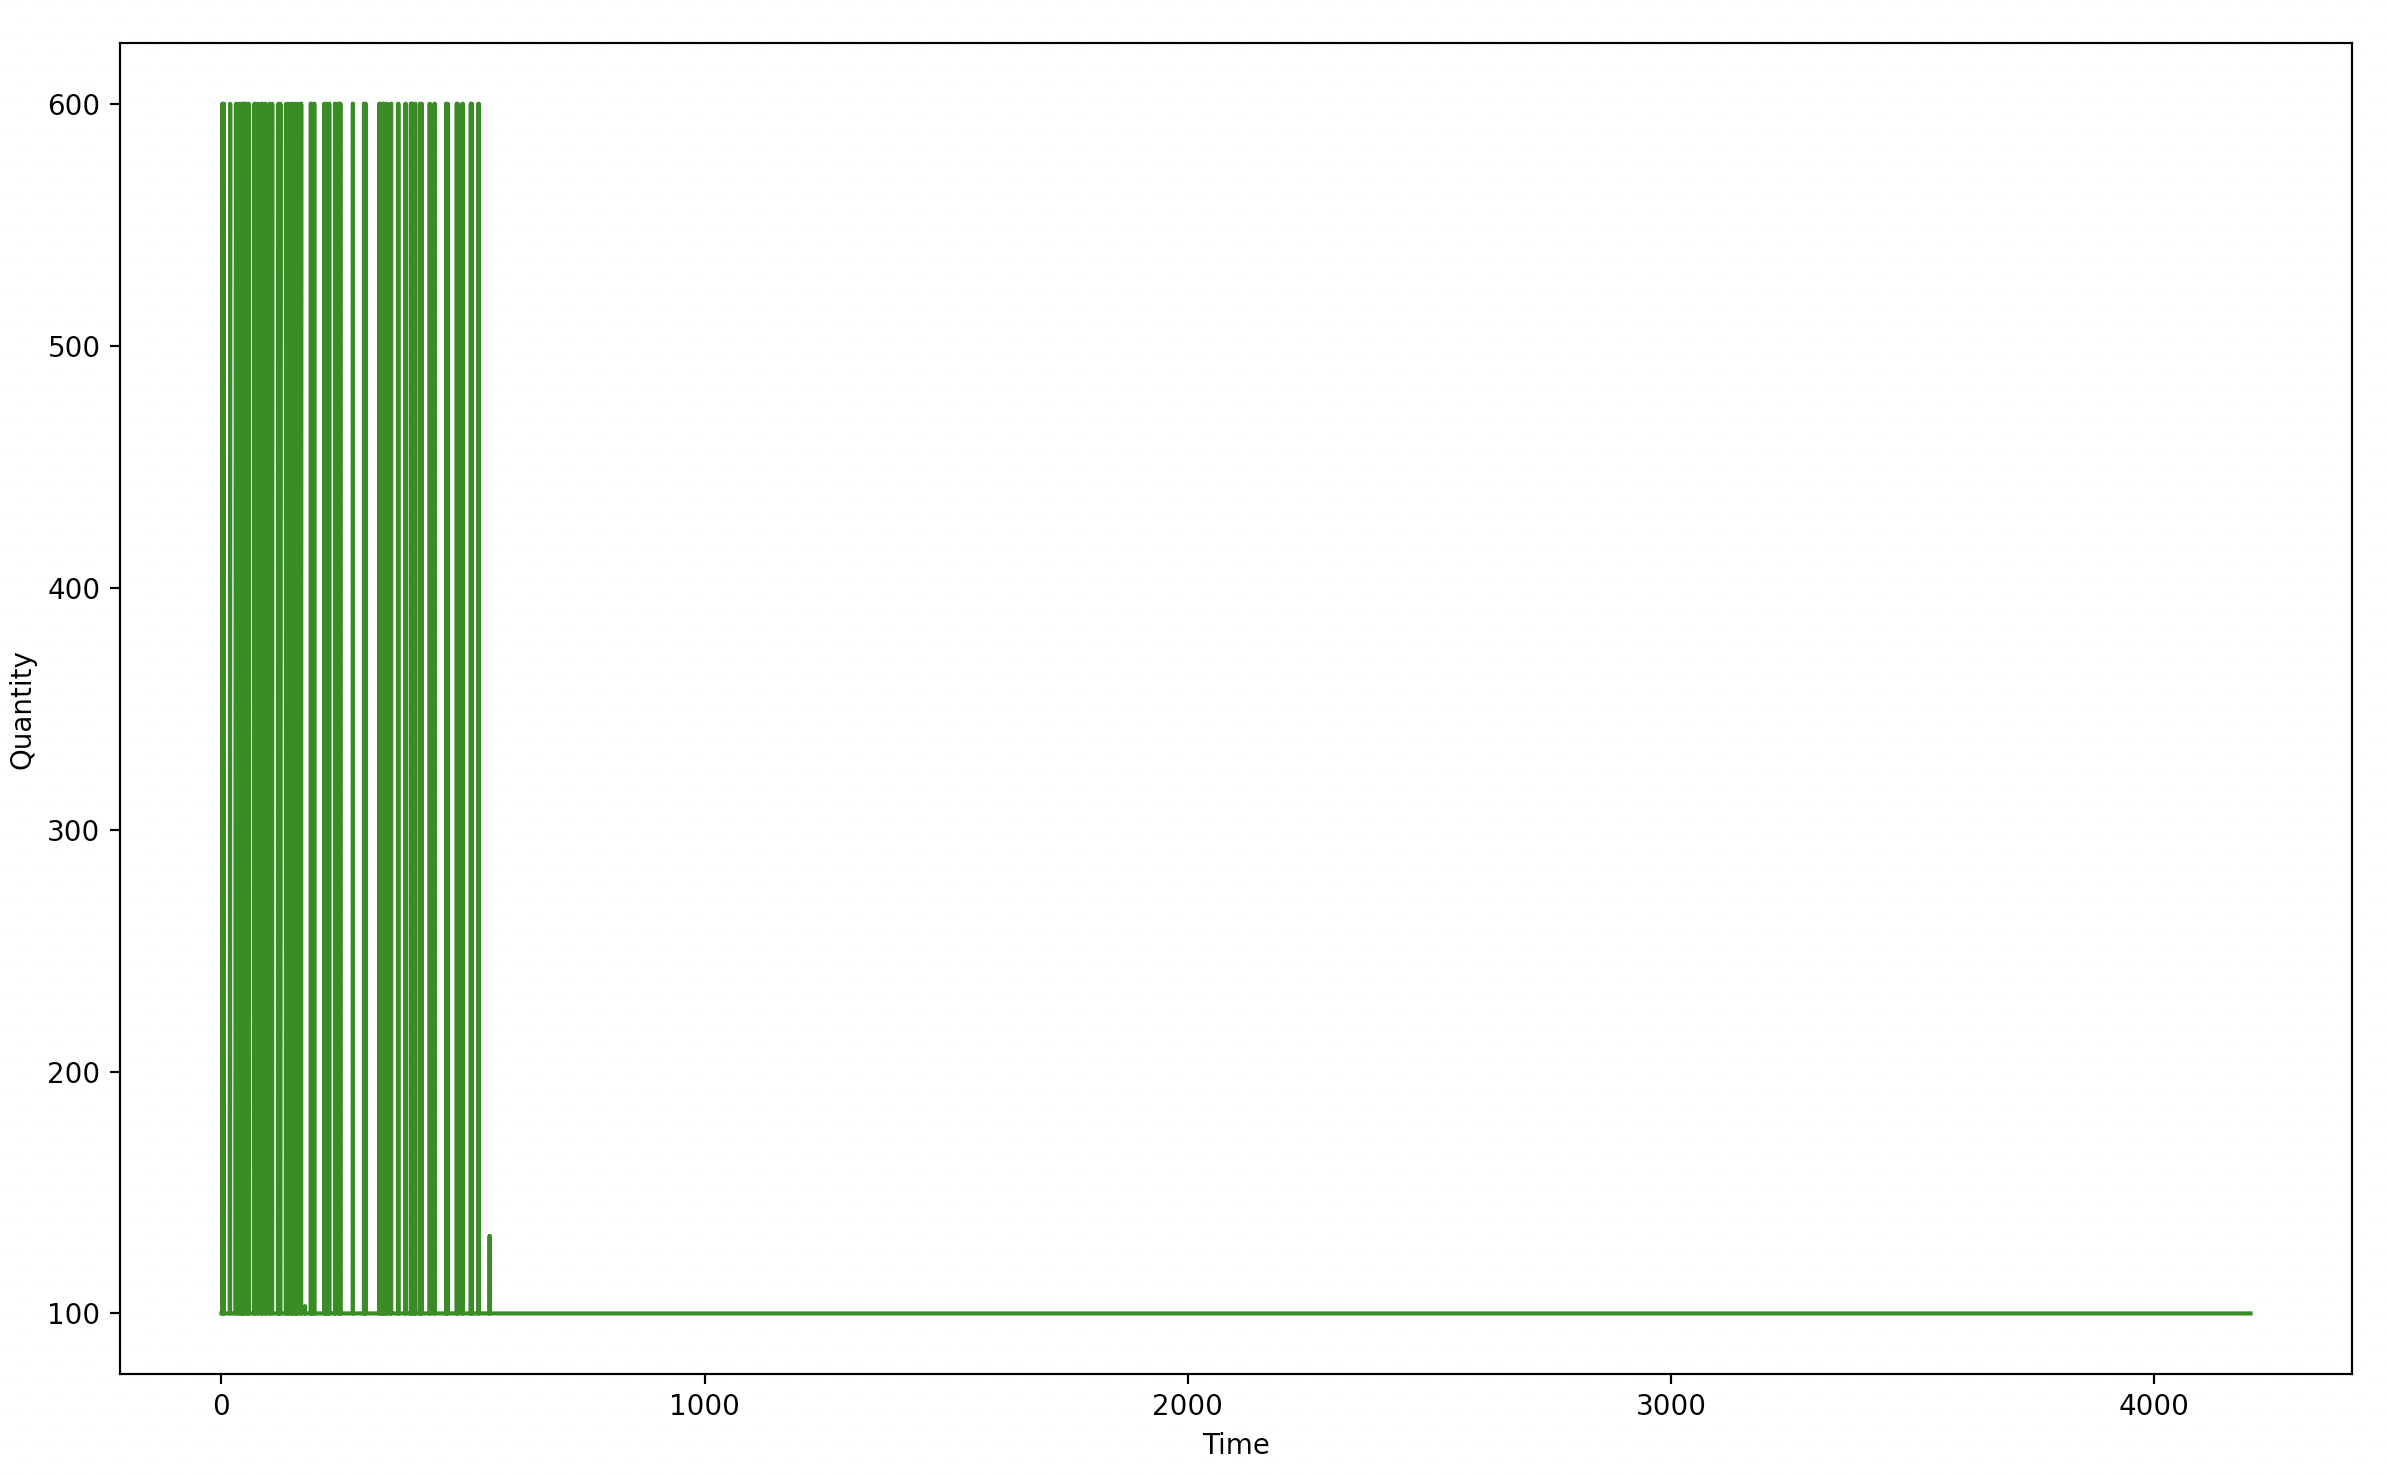
\includegraphics[width=7cm, height=6cm]{Dissertation/images/mcg_indv/LIQ/100.png}
    \caption{Simple seller quantity of 100}
    \label{fig:1}
  \end{subfigure}
  %
  \begin{subfigure}[b]{0.5\textwidth}
    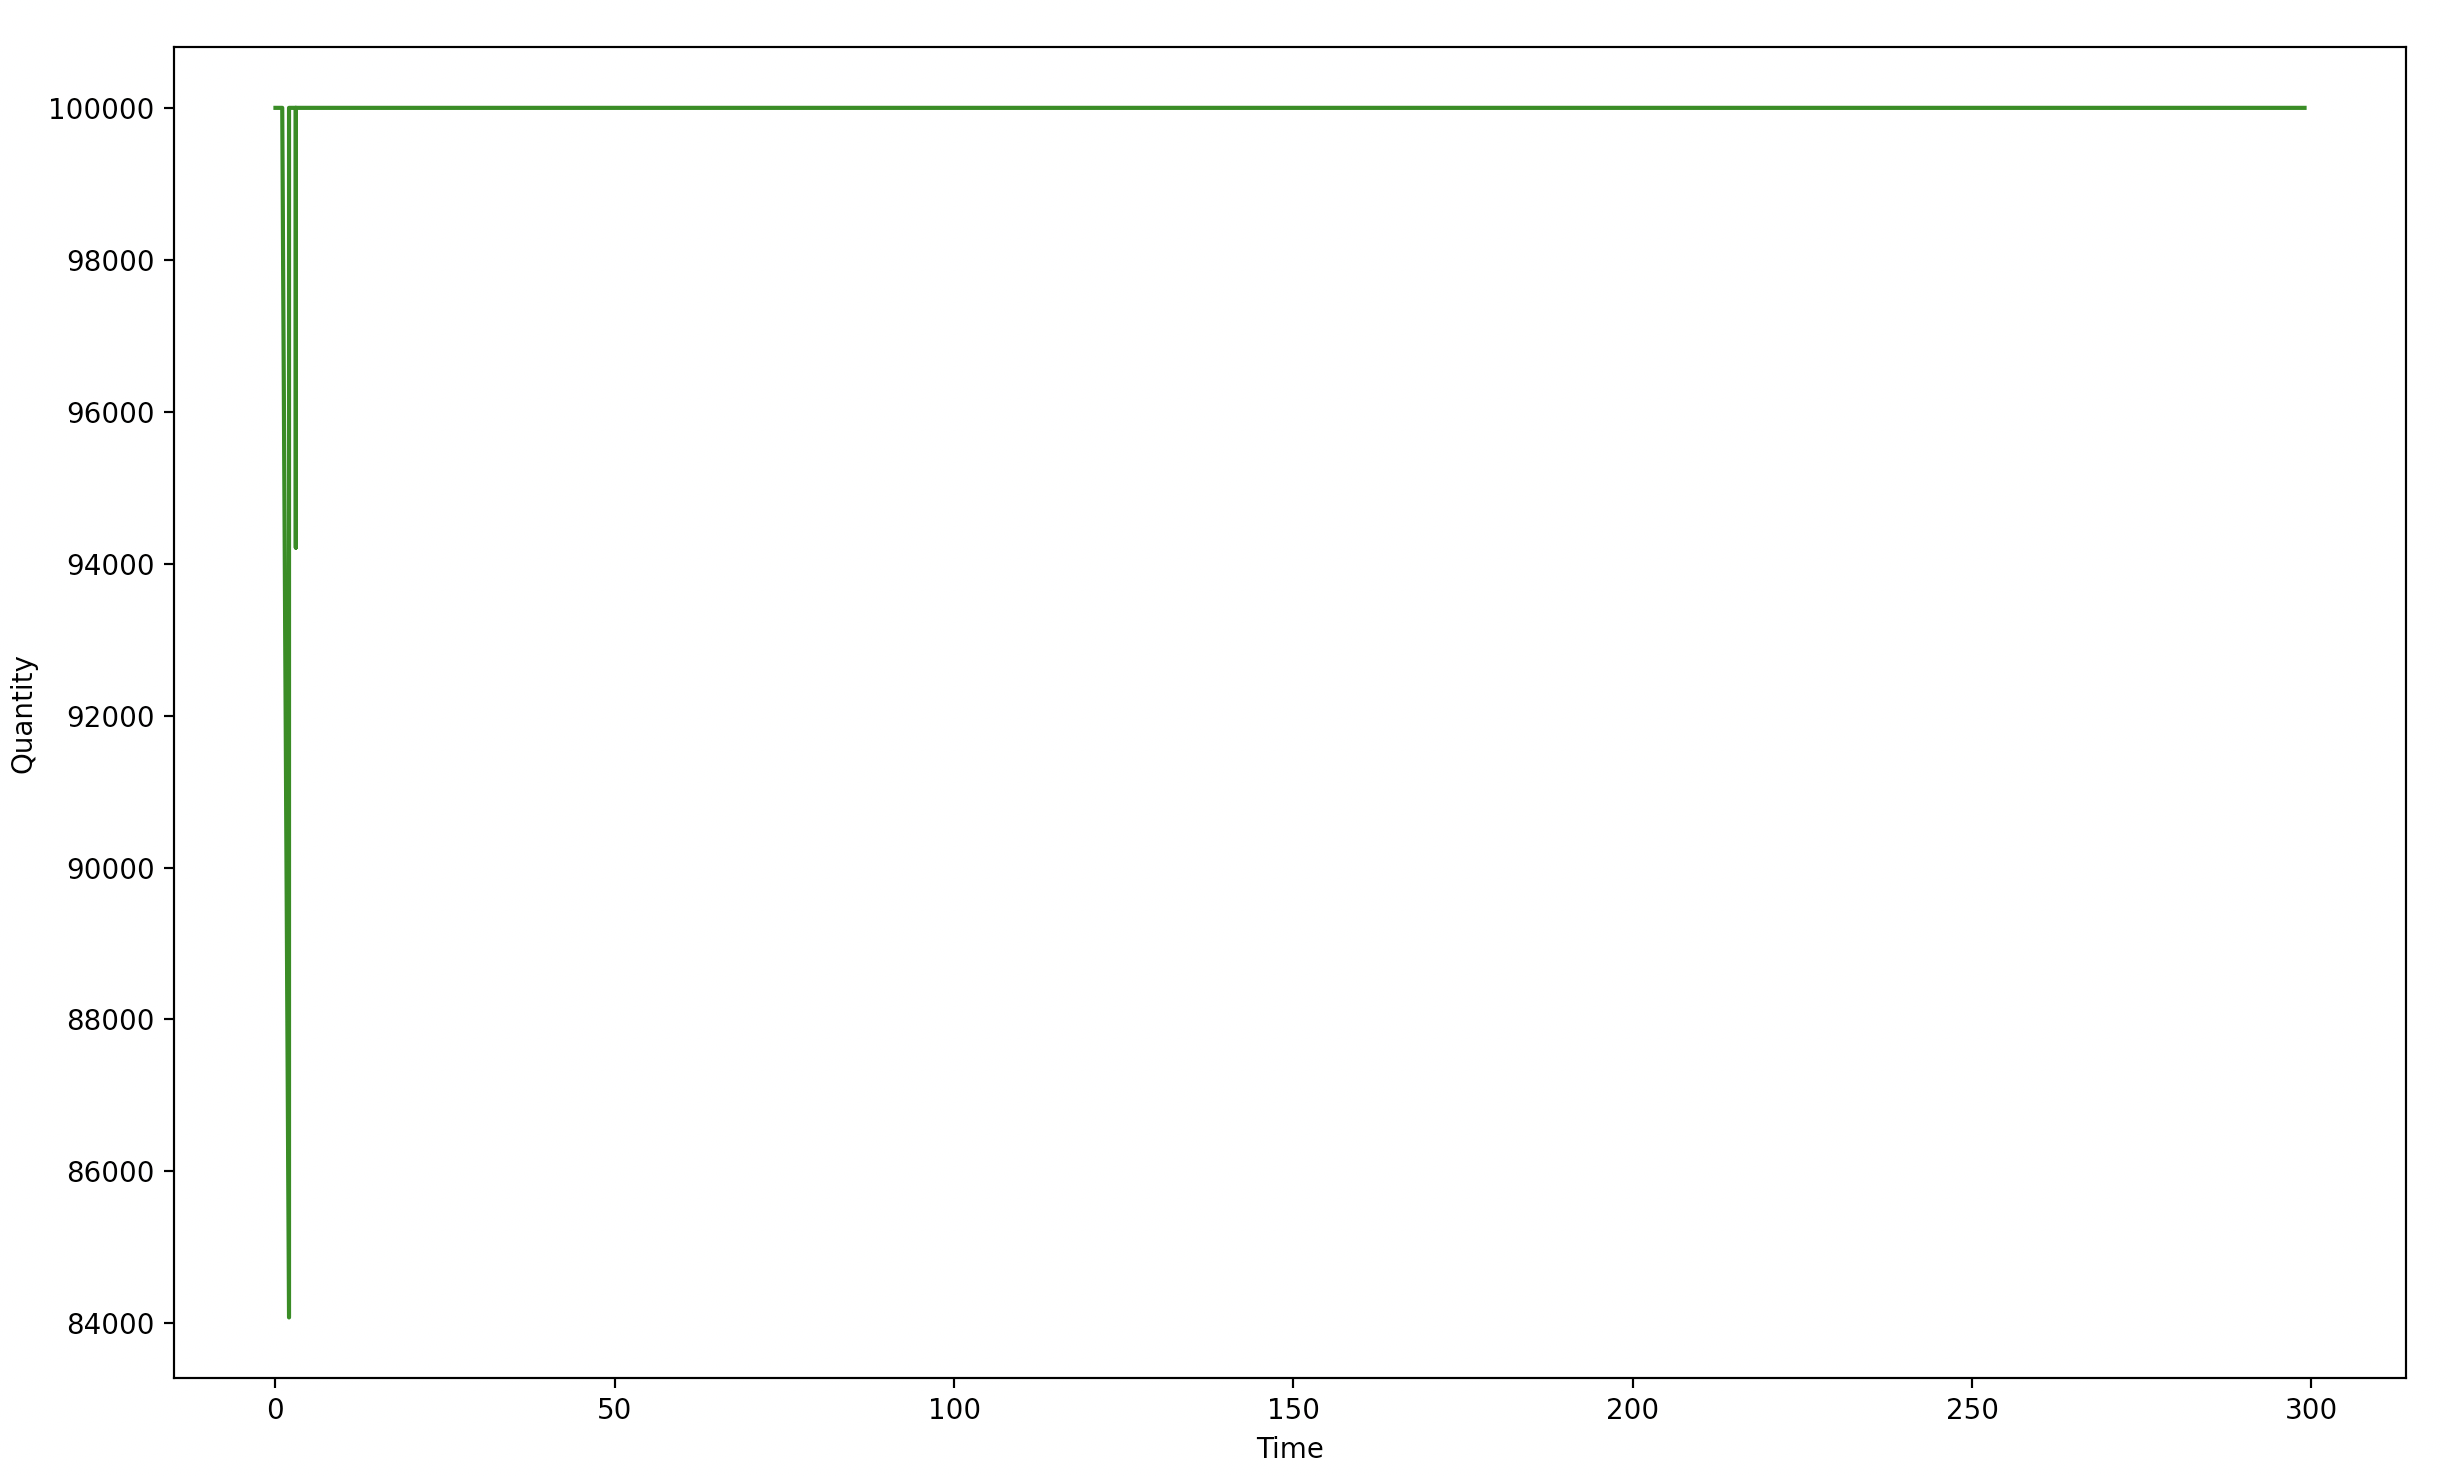
\includegraphics[width= 7cm, height=6cm]{Dissertation/images/mcg_indv/LIQ/san.png}
    \caption{Simple seller quantity of 100,000}
    \label{fig:2}
  \end{subfigure}
\caption{Quantity of all orders submitted : Liquidity consumer with Simple Seller submitting different quantity of orders} 
\end{figure}

The first case in figure 5.2(a) is when the Simple sellers are only submitting at $price = 100$ and $quantity = 100$. The test ran with 4200 McG time period in order to illustrate the orders submitted. It can be seen that in the initial period of the market, the orders submitted mostly is 600. This is because the Liquidity consumer is submitting the best quantity of the best price of the opposite side of the book (which is $price = 100$ and quantity = $ 100 * number of Simple sellers$). In addition, only the Liquidity consumer that is randomized with a ``bid" as their task of the day is only submitting because the ``ask" Liquidity traders cannot submit. This is because there is no Limit orders in the bid side of the book since the only bid orders are market orders submitted by other Liquidity consumers.

The second case in figure 5.2(b) is when Simple sellers are submitting at $price = 100$ and $quantity = 100,000$. The test is run with 300 McG action step to better illustrate the initial results of the market. This means that the ``ask" day task Liquidity traders will submit their initial large order and then stop after submitting one order. In addition, because the Liquidity trader has 0.1 probability of acting, only 3 agents submitted their orders, which is the three lower spikes seen in the initial time period of the market. The rest of the orders seen in the market at 100,000 quantity is from Simple Sellers. Similar results can be seen with Simple Buyer in similar experiments. 

\section{Momentum trader}
The momentum trader is one of the high frequency trader who will "play along with the tide". The agent will submit an ask order if the price has been recently falling and a bid if the price has been recently rising. 

\begin{table}[h]
\centering
\begin{tabular}{ |m||p{4cm}|} 
\hline
\textbf{Momentum trader Parameters}& \textbf{Value} \\
\hline
\hline
$n_r$ & 5 \\ 
\hline
$\kappa$ & 0.001\\ 
\hline
$V_{mt}$ & 5,000,000 (100,000 in the test) \\ 
\hline
\end{tabular}
\caption{Momentum trader parameters taken from \cite{McGroarty}} 
\end{table}
\FloatBarrier 

\subsection{Momentum trader's Wealth}
One of the important variable in the Momentum trader's trading strategy is its wealth. The agent will submit the quantity of an order based on its wealth given by equation : $v_t = \abs{roc_t} * W_{a,t}$. The concept of Wealth $W_{a,t}$ is different in this BSE implementation due to the fact that the agent can submit either a bid or an ask in any order. In reality, a trader can submit an ask (playing short) then buy back the stocks at a later date. Similarly, one can buy a quantity of stock and sell it back at a later date. Because the Momentum trader does not have that constraint, there must be some abstraction in calculation of wealth. 

The approach taken in this project is follow: The wealth will be separated into two types : Ask balance and Bid balance. 

\begin{itemize}
  \item \textbf{Ask Balance} : The initial price is 0. This is due to the fact that if someone sells a product, their wealth will increase. After the agent's market order is fulfilled, their ask balance will increase by $quantity * price_{transaction}$. This idea is abstracted from the fact that the agent can sell something it does not have. The ask balance will be capped at $V_{mt}$. 
  \item \textbf{Bid Balance} : The initial price is $V_{mt}$. This is due to the fact that if someone buys a product, their wealth will decrease. After the agent's market order is fulfilled, their bid balance will decrease by $quantity * price_{transaction}$. The bid balance will be capped at 0.
\end{itemize}

The wealth $W_{a,t}$ of the agent is then calculated by Ask balance + Bid balance. 

\subsection{Momentum trader Test} 
Similar to Liquidity consumer, the Momentum trader submits only a market order. Hence, in the following experiment, only the quantity and the type of order will be investigated.  

The experiment will consists with two types of price arrangement : increasing and decreasing. This is to investigate whether the momentum trader will respond correctly to the momentum in the price. In order to evaluate the current Mean Reversion algorithm, the following test will be conducted. The Simple Seller and Buyer will be modified such that:
\begin{itemize}
  \item It will include a probability of submitting at 0.25 to ensure that the orders don't always match and there is limit orders left in the Limit Order book. 
  \item The agents will submit with quantity drawn uniformly from between 100 and 1000 to ensure that the Limit Order Book is not empty
  \item The agents will submit either a decreasing or increasing price in each iteration. For example, if it is decreasing, the initial price will be 1000 and decremented by 1 in each McG action step. This ensures that the mid price will be a downward slope and the momentum of the market is in the downward slide. 
\end{itemize}

The experiment will run in 1000 McG action step. The market consists of 6 Simple Buyers, Simple Sellers and Momentum trader. The results are illustrated below: 

\begin{figure}[h]
  \begin{subfigure}[b]{0.5\textwidth}
    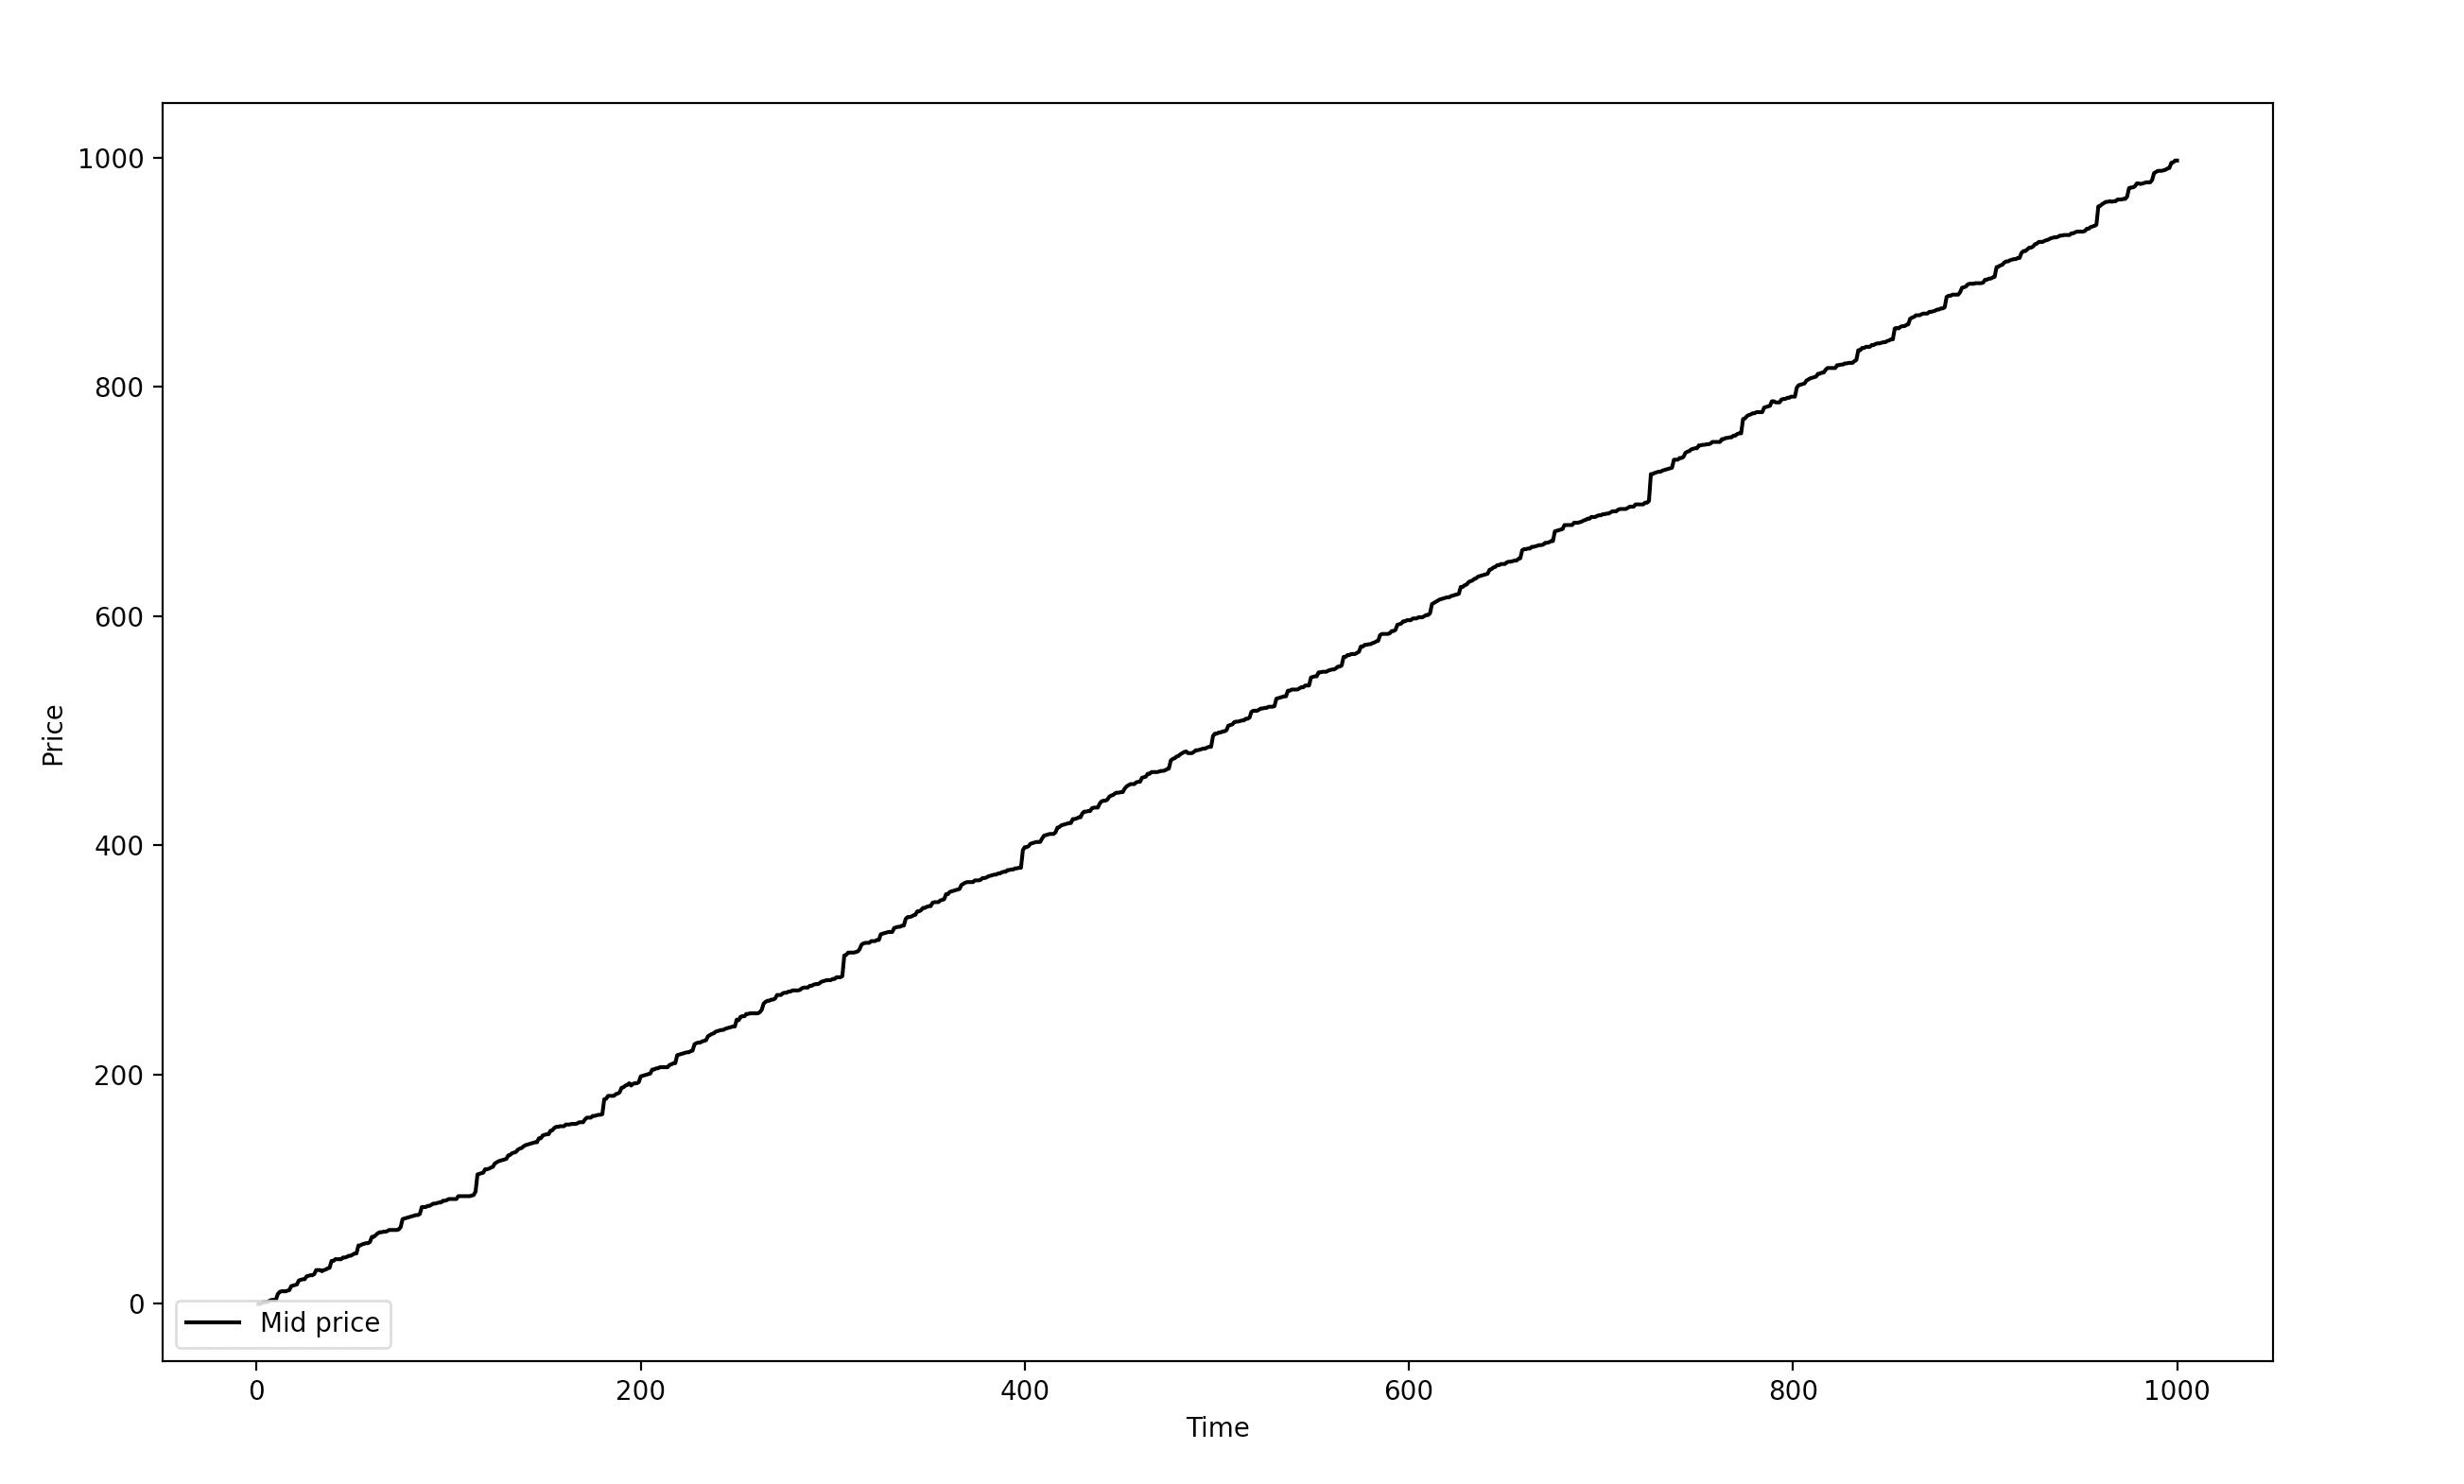
\includegraphics[width=7cm, height=6cm]{Dissertation/images/mcg_indv/MMT/incr.png}
    \caption{Mid Price}
    \label{fig:1}
  \end{subfigure}
  %
  \begin{subfigure}[b]{0.5\textwidth}
    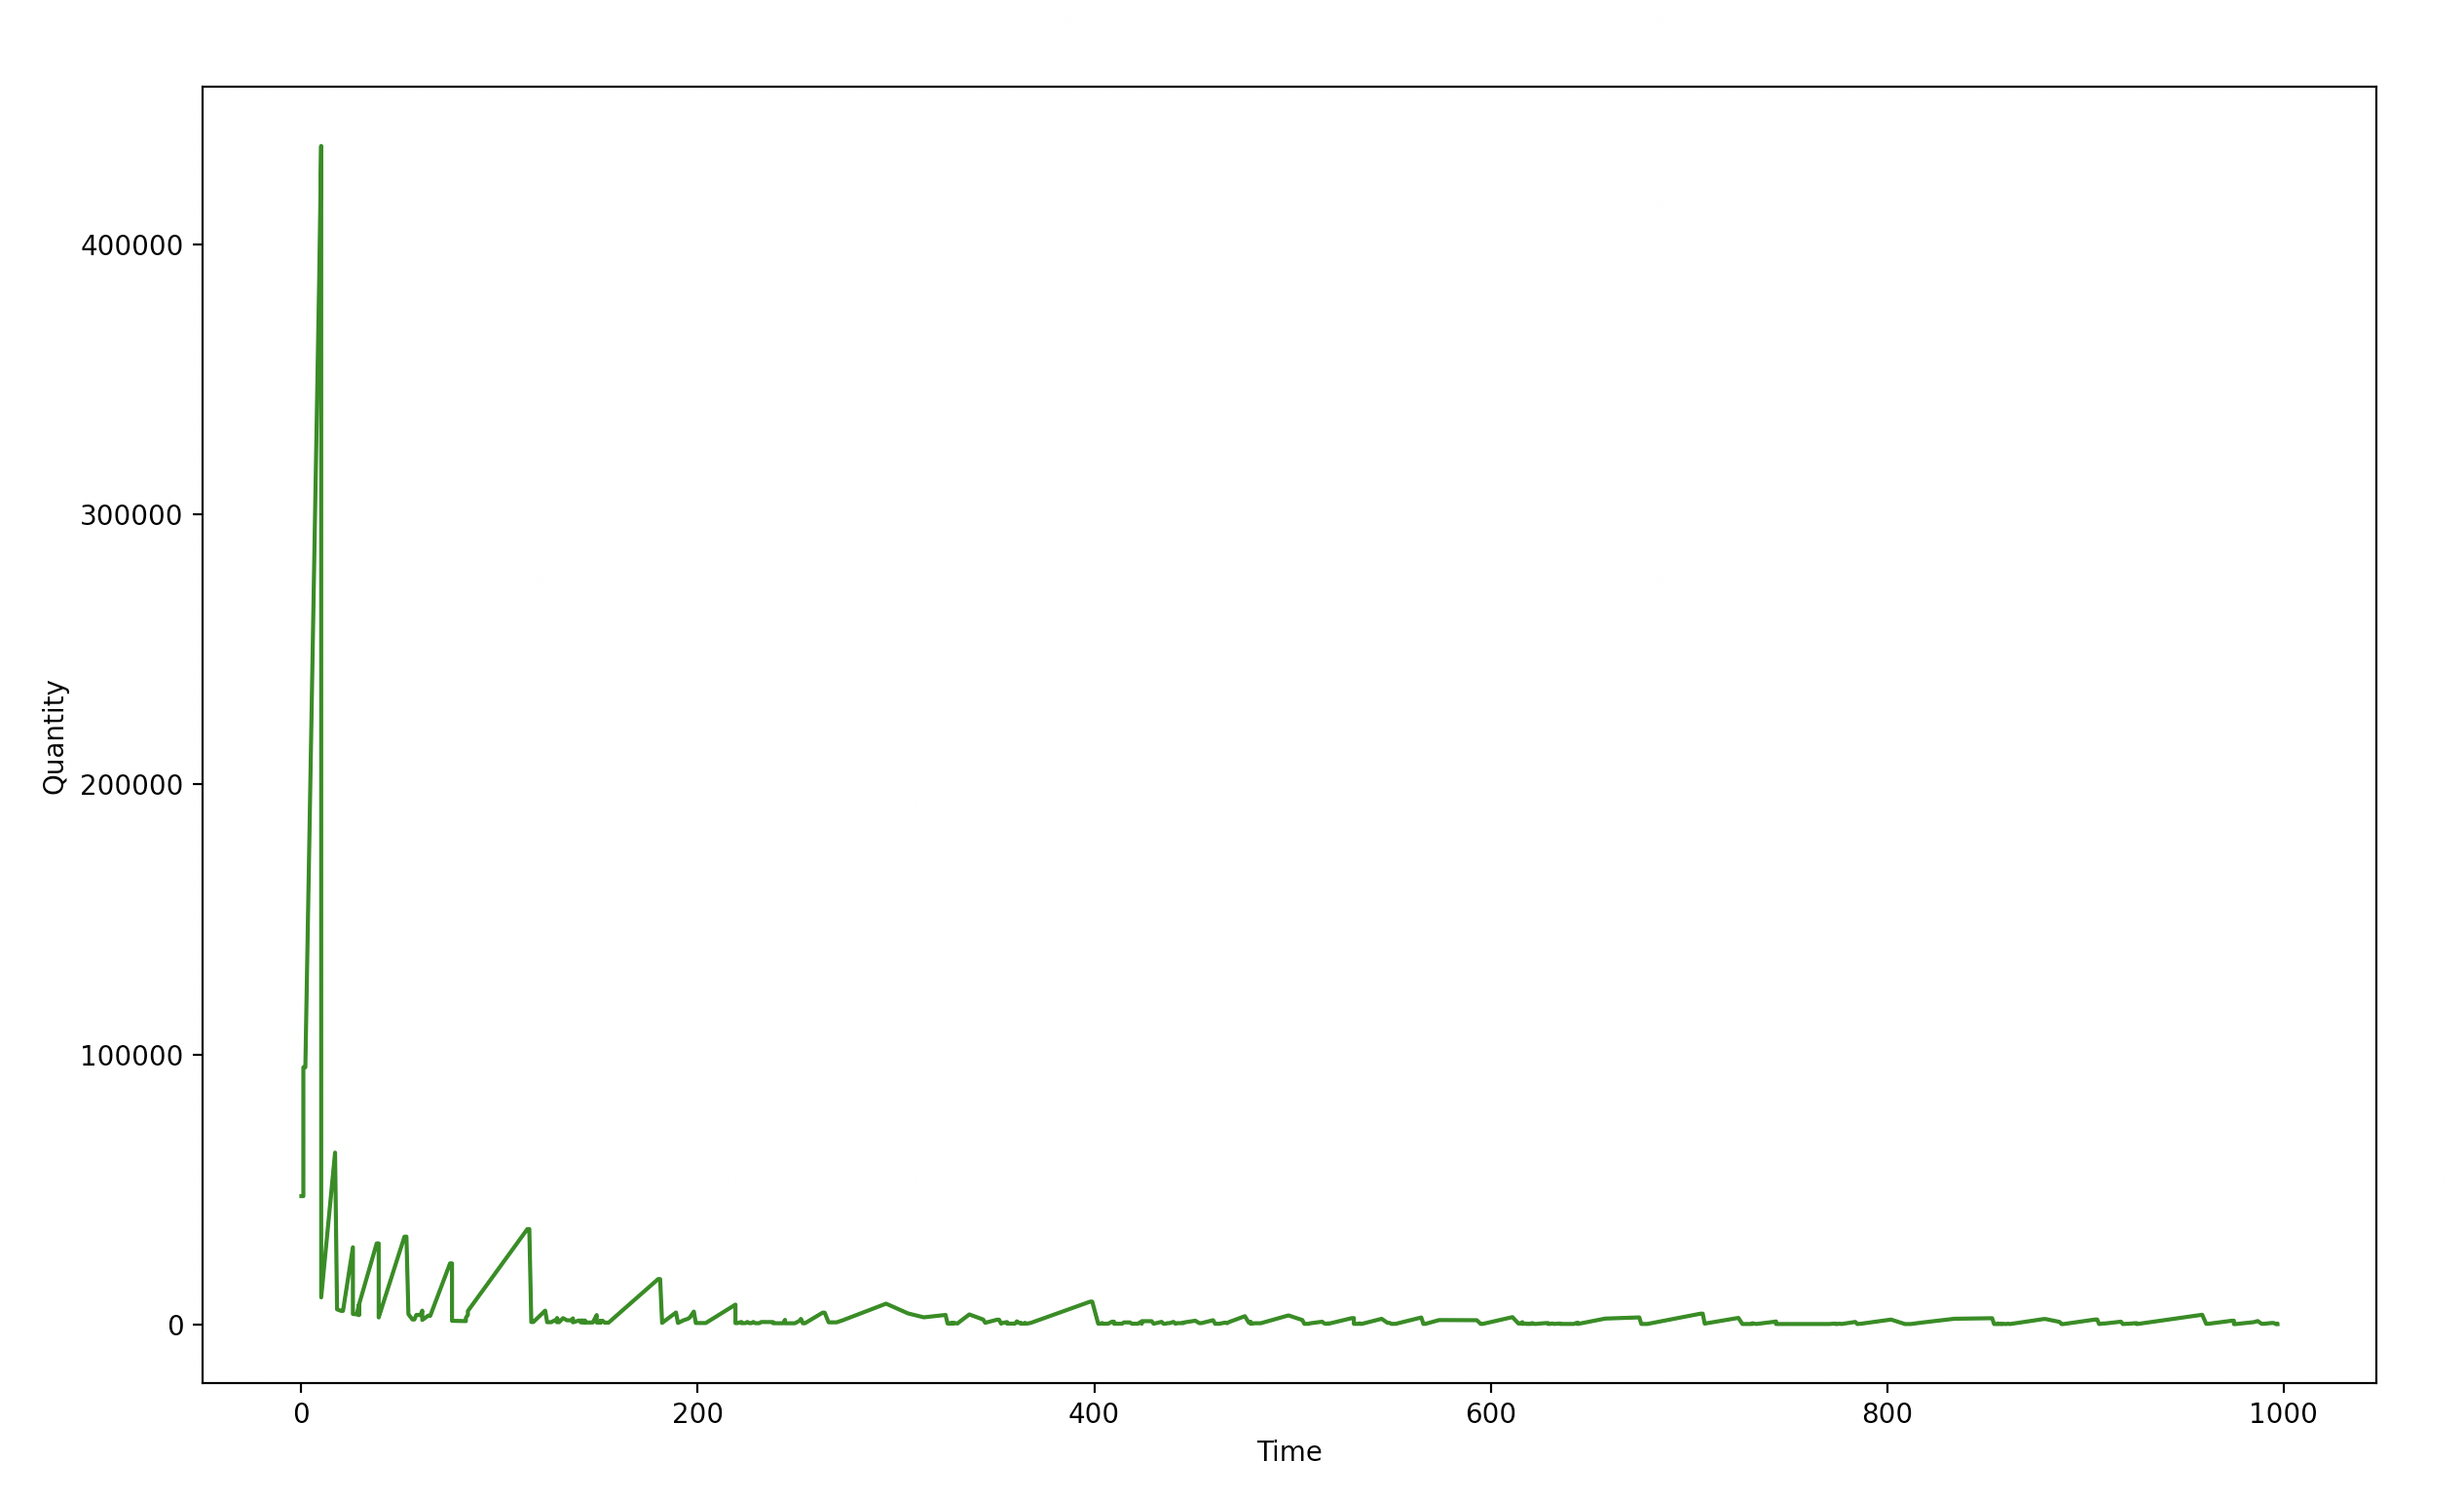
\includegraphics[width= 7cm, height=6cm]{Dissertation/images/mcg_indv/MMT/incr_qty.png}
    \caption{Quantity submitted by Momentum trader}
    \label{fig:2}
  \end{subfigure}
\caption{Momentum trader increasing price experiment} 
\end{figure}


\begin{figure}[h]
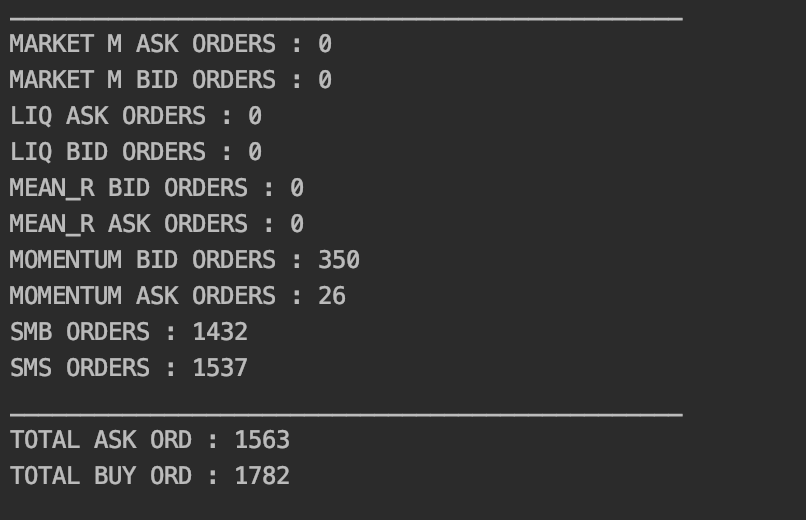
\includegraphics[ height=8cm]{Dissertation/images/mcg_indv/MMT/incr_stat.png}
\caption{Momentum trader increasing price experiment statistics} 
\end{figure} 
\FloatBarrier

The figures above illustrate the increasing test results of the market. Figure 5.3(a) illustrates the mid price which increases over the 1000 time period. The quantity submitted by agents will quickly decrease because of the reduction in its wealth because it is only buying and not selling. The majority of the order submitted in figure 5.4 will be bid orders because the market is gaining an upward momentum. 

\begin{figure}[h]
  \begin{subfigure}[b]{0.5\textwidth}
    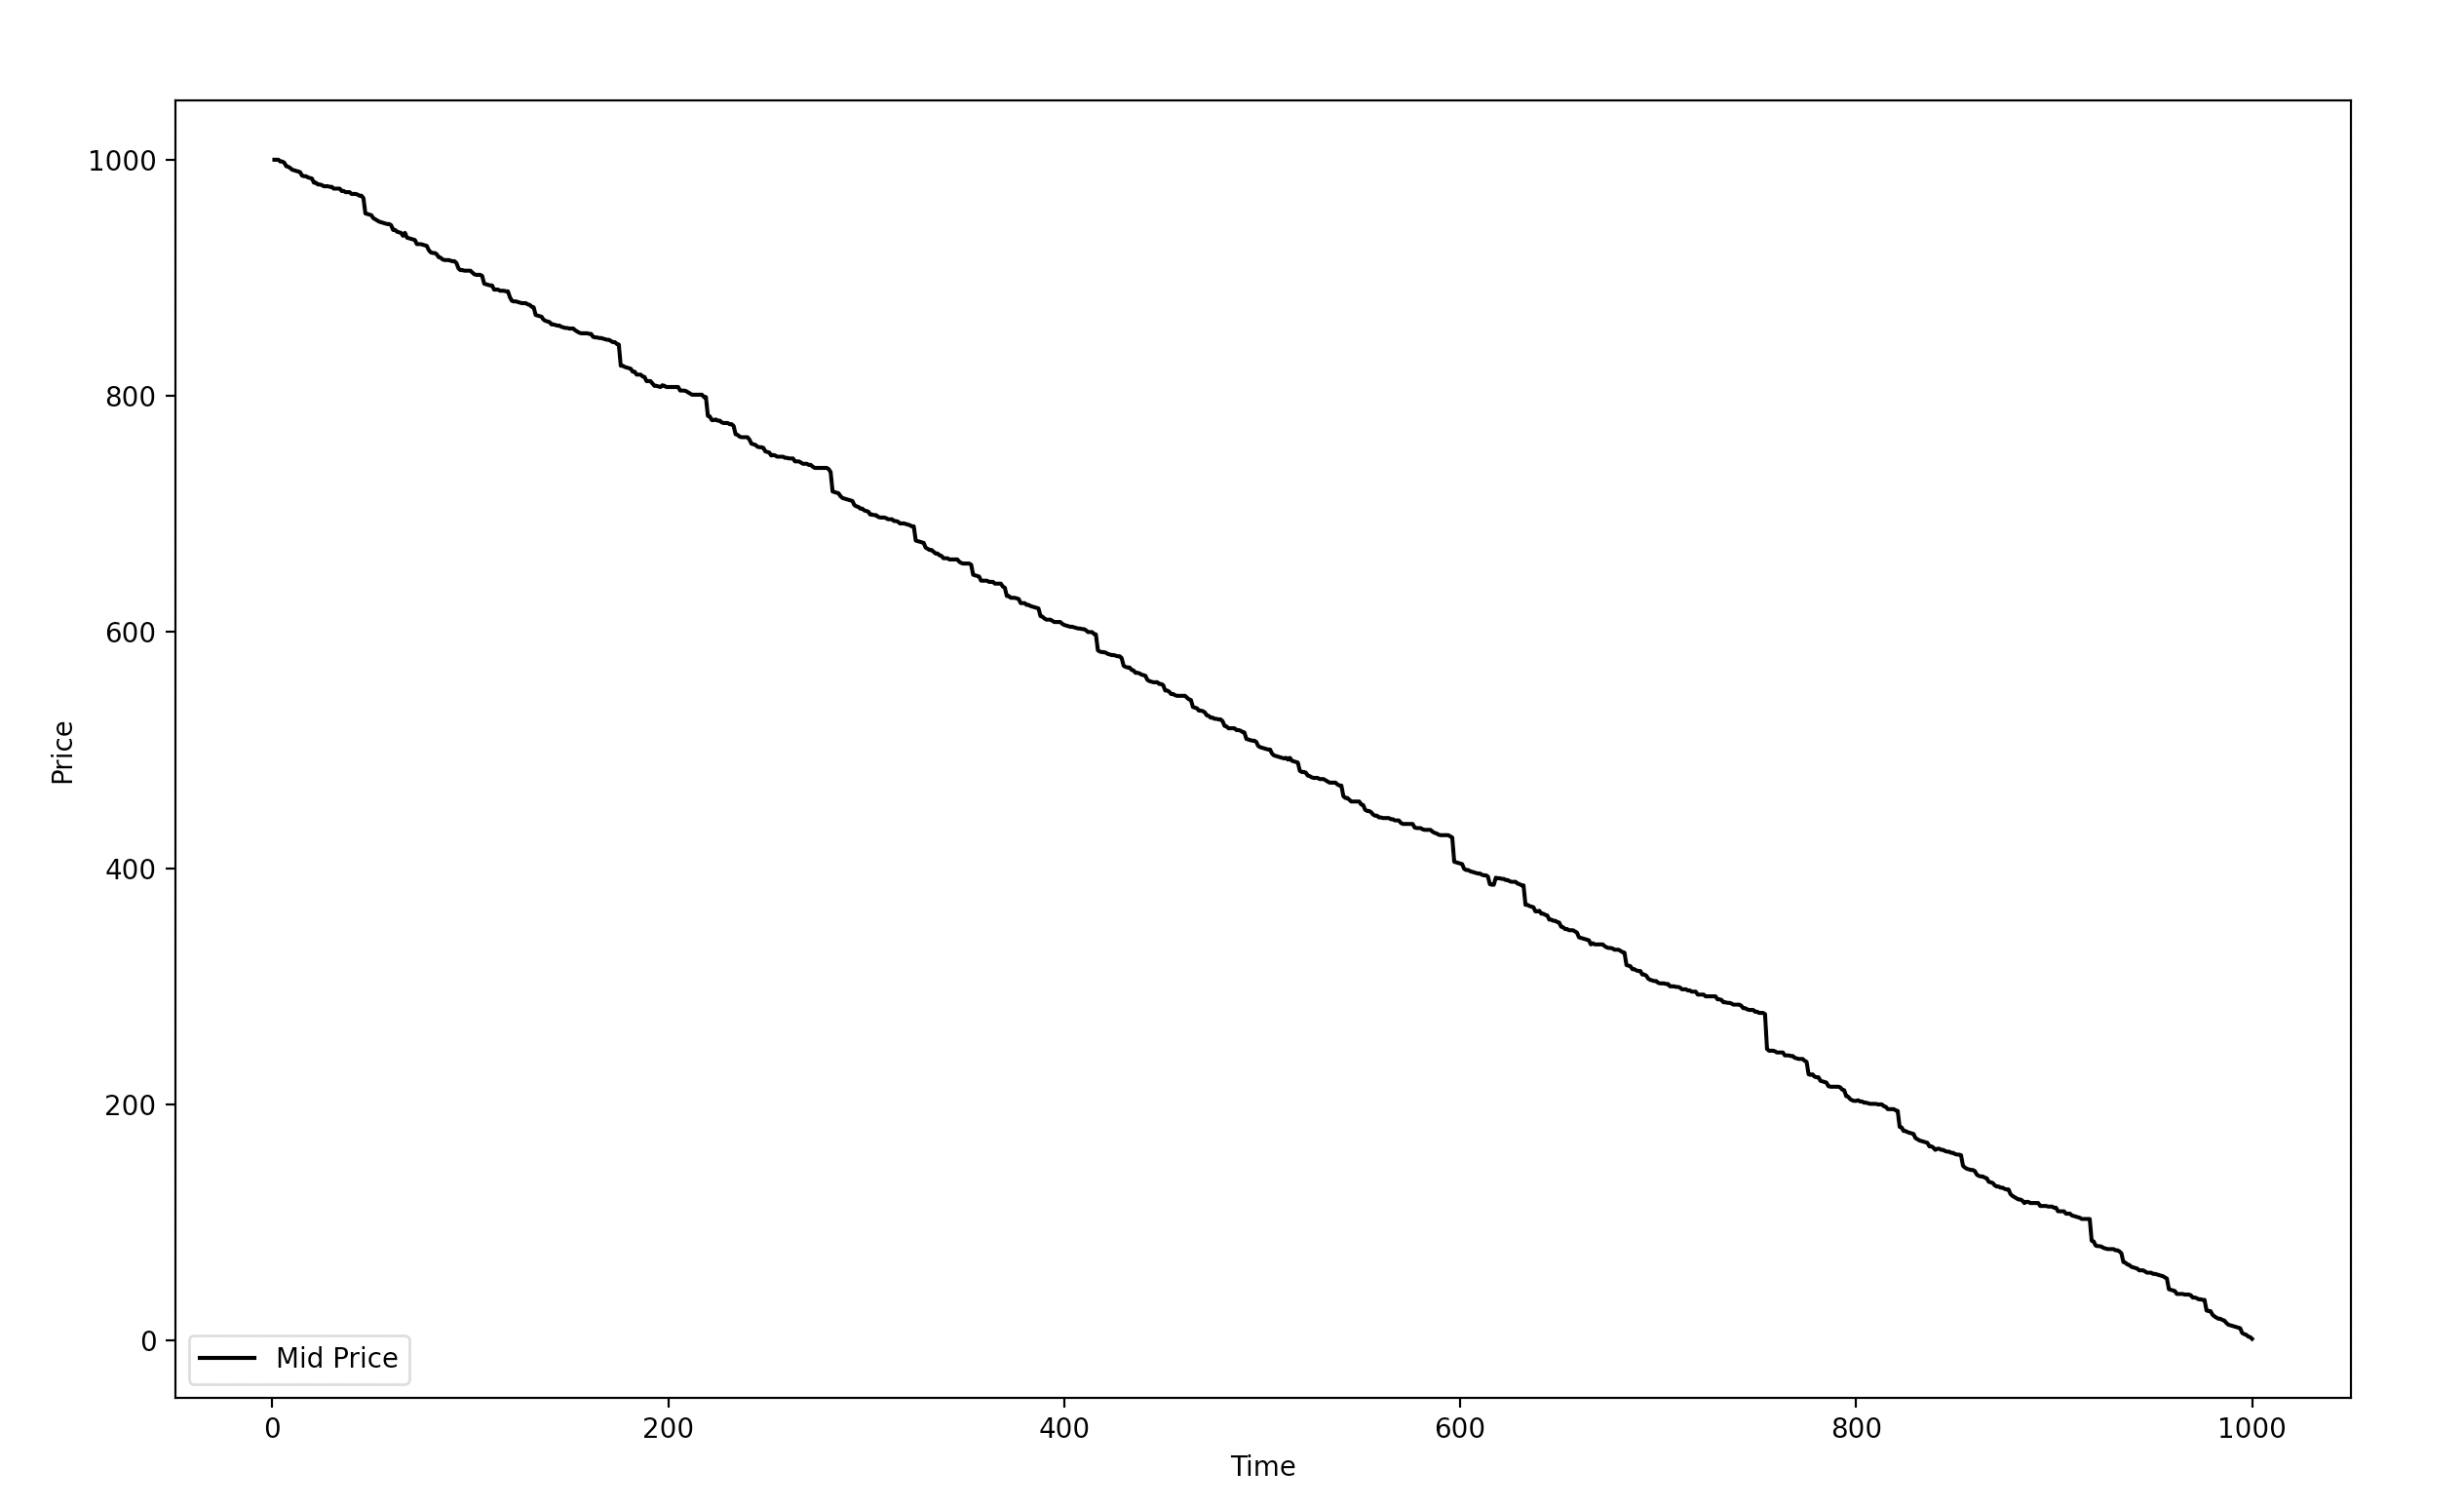
\includegraphics[width=7cm, height=6cm]{Dissertation/images/mcg_indv/MMT/dec_price.png}
    \caption{Mid Price}
    \label{fig:1}
  \end{subfigure}
  %
  \begin{subfigure}[b]{0.5\textwidth}
    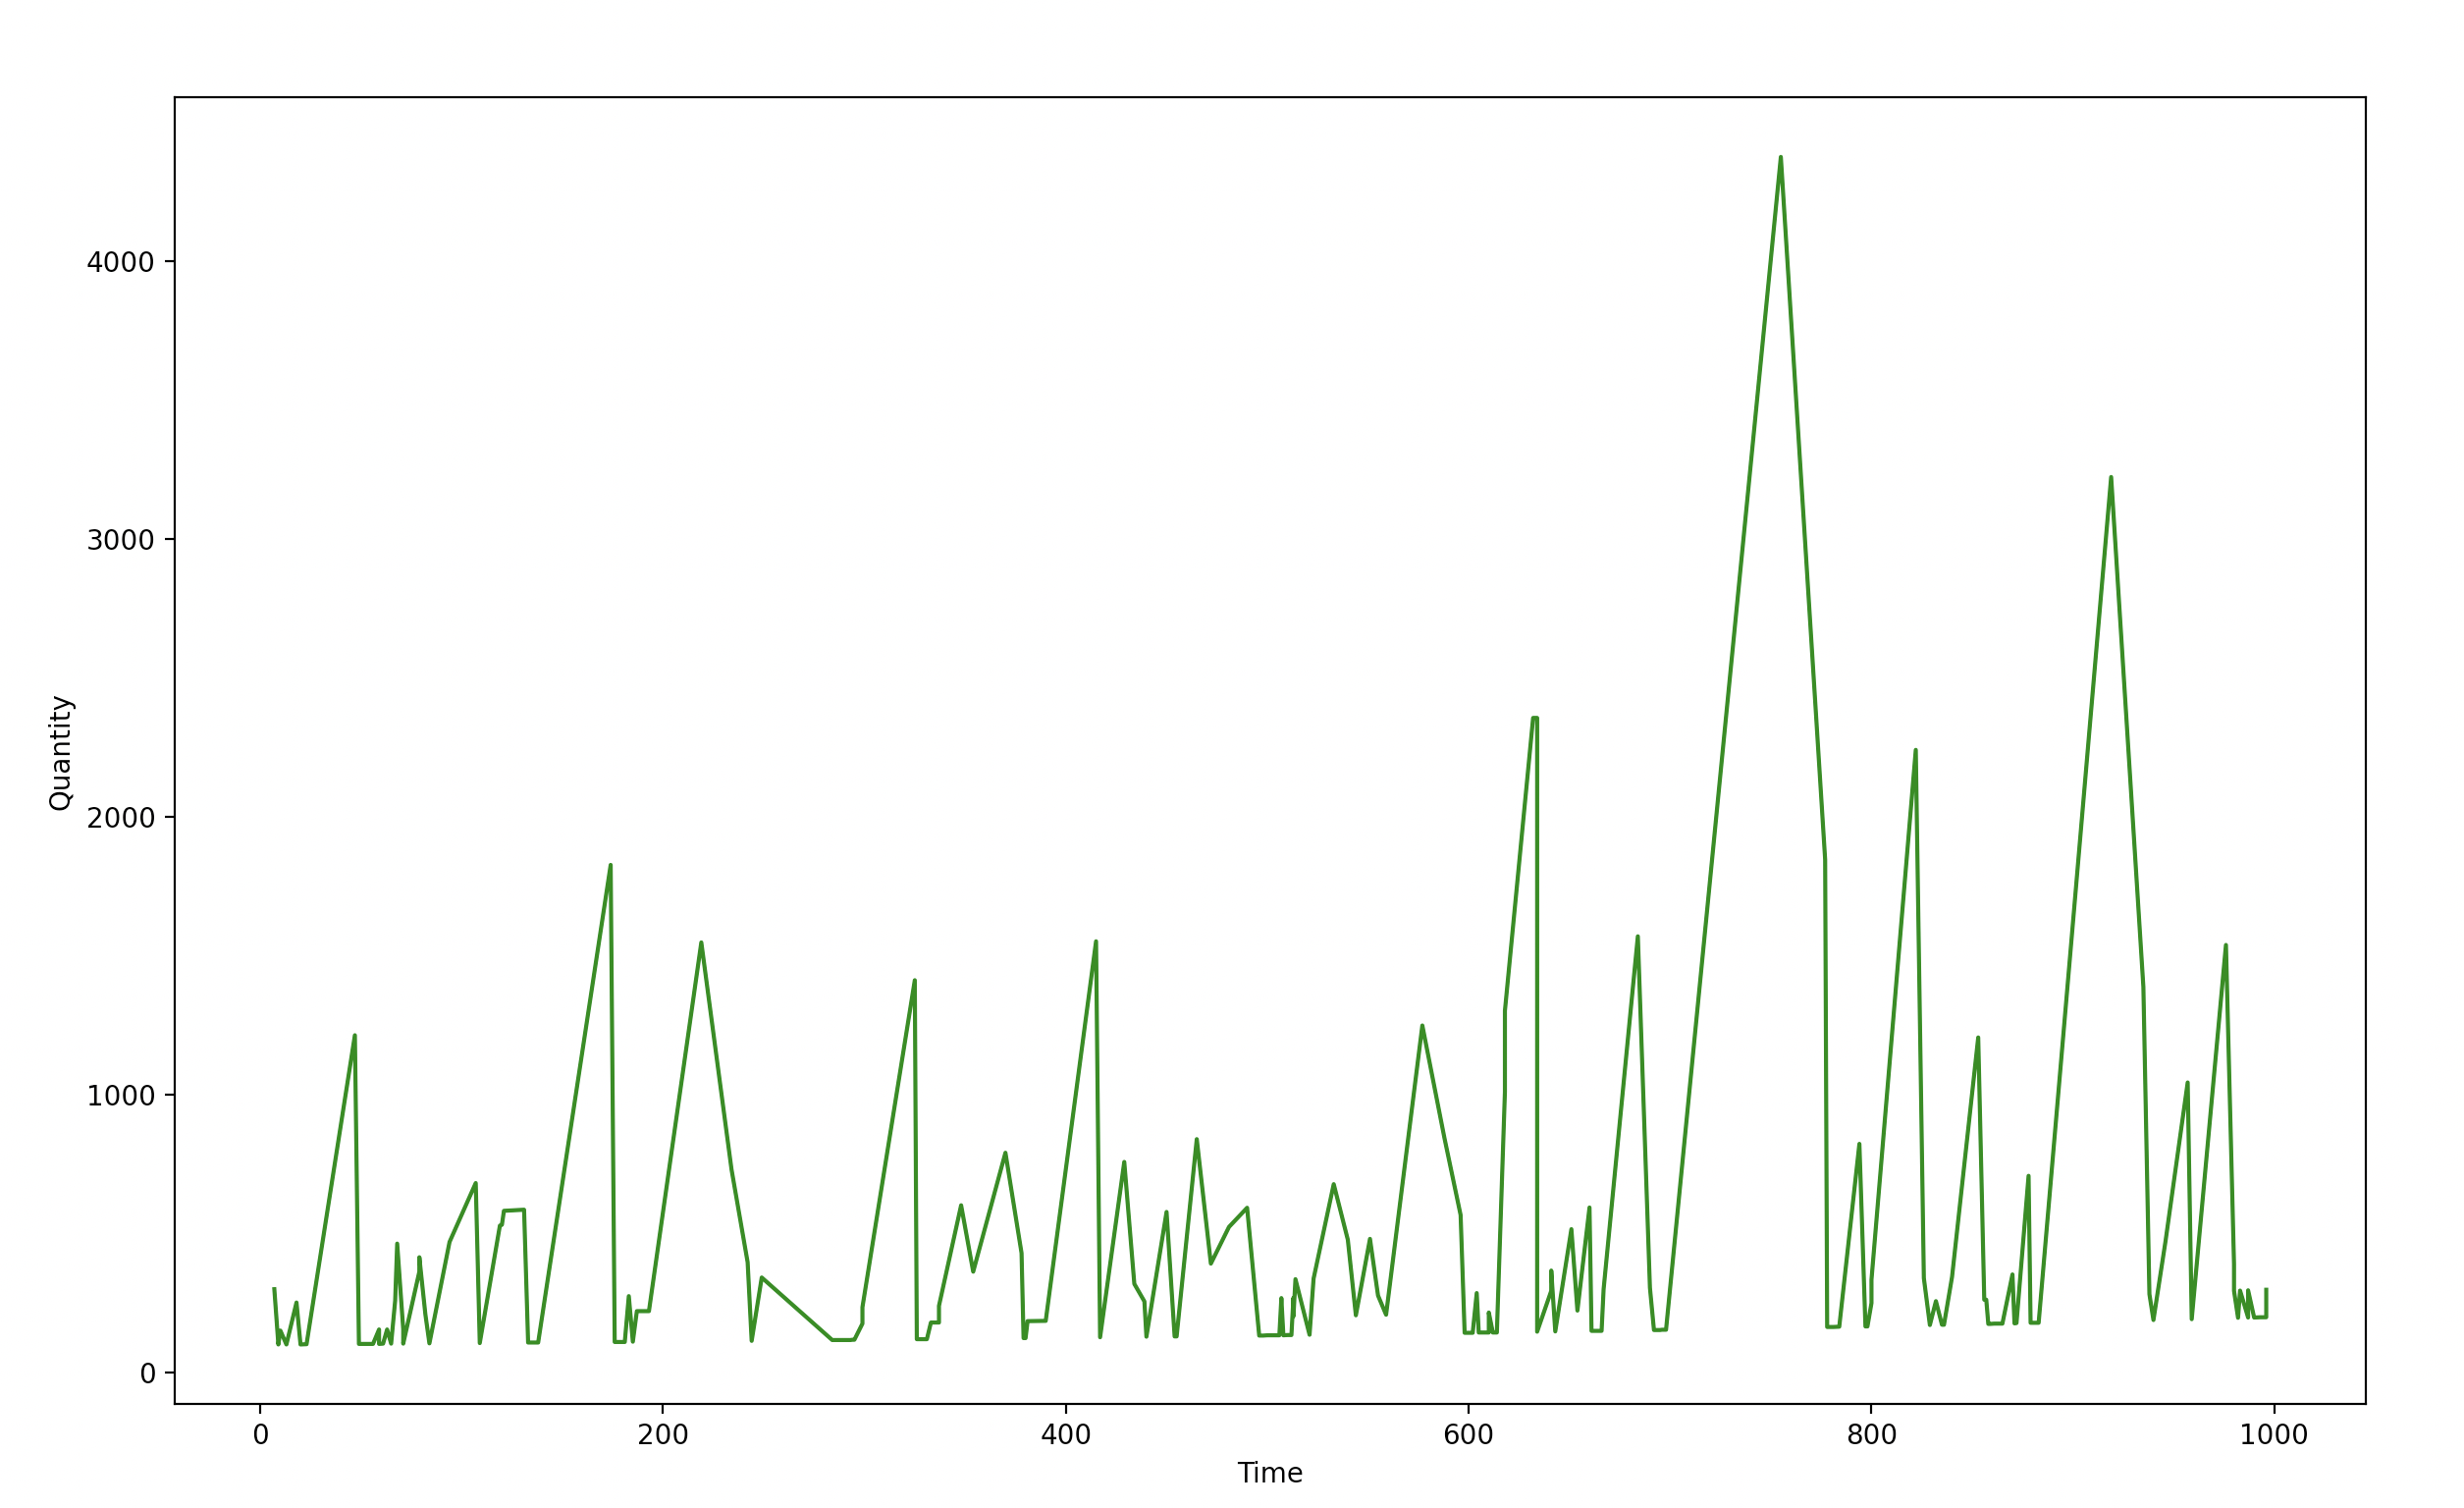
\includegraphics[width= 7cm, height=6cm]{Dissertation/images/mcg_indv/MMT/dec_qty.png}
    \caption{Quantity submitted by Momentum trader}
    \label{fig:2}
  \end{subfigure}
\caption{Momentum trader decreasing price experiment} 
\end{figure}


\begin{figure}[h]
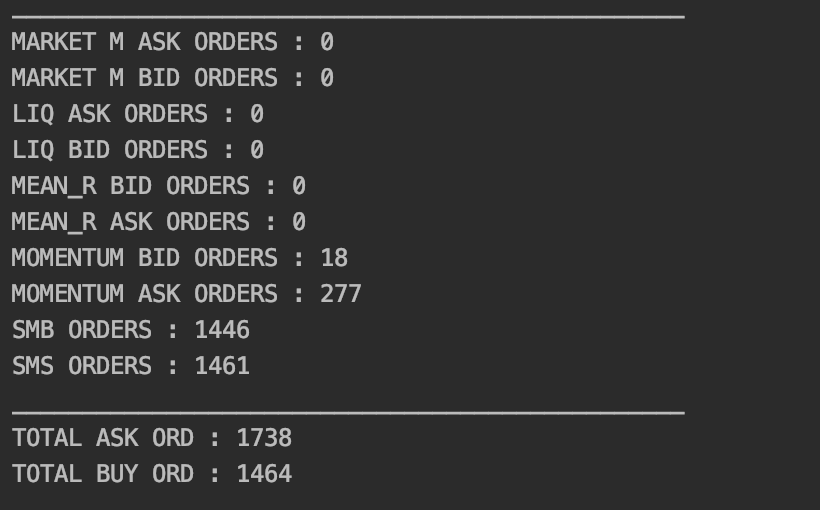
\includegraphics[ height=8cm]{Dissertation/images/mcg_indv/MMT/dec_stat.png}
\caption{Momentum trader decreasing price experiment statistics} 
\end{figure} 
\FloatBarrier

The figures above illustrate the decreasing test results of the market. Figure 5.5(a) illustrates the mid price which decreases over the 1000 time period. The quantity of this experiment is different since the agents are submitting only ask orders, hence their wealth is increasing over time. This means that their quantity submitted will also increase, as seen where there is a huge spike in order over 4000 in near the $800^{th}$ iteration. The majority of the order submitted in figure 5.4 will be asks orders because the market is gaining an downward momentum. 

\section{Mean reversion trader}
The Mean reversion trader is intended to represent one type of a high frequency trader who believes that the price of the market will always revert back to the rolling-average line. The mean reversion behaviour is better illustrated with a simpler unit test with no other agents in the market.

\begin{table}[h]
\centering
\begin{tabular}{ |m||p{4cm}|} 
\hline
\textbf{Mean Reversion consumer Parameters}& \textbf{Value} \\
\hline
\hline
$v_{mr}$ & 1 \\ 
\hline
$\alpha$ & 0.94\\ 
\hline
$k$ & 1 \\ 
\hline
$w_{mr}$ & 50 (10 in the experiment)\\ 
\hline
\end{tabular}
\caption{Mean Reversion consumer parameters taken from \cite{McGroarty}}  
\end{table}
\FloatBarrier

In order to evaluate the current Mean Reversion algorithm, the following test will be conducted. The Simple Seller and Buyer will be modified such that:
\begin{itemize}
  \item It will include a probability of submitting at 0.25 to ensure that the orders don't always match and there is limit orders left in the Limit Order book. 
  \item The agents will submit with quantity drawn uniformly from between 100 and 1000 to ensure that the Limit Order Book is not empty
  \item The agents will submit a random price drawn uniformly between 98 to 102. This is to mimic the price range that will be seen in the real McG experiment. 
\end{itemize}

The following experiment will run for 50 McG time period. The market consists of 1 Mean Reversion trader, 6 Simple Buyer and 6 Simple Seller. The graph represents the behaviour of a single agent in detail. The results are illustrated below. 

\begin{figure}[h]
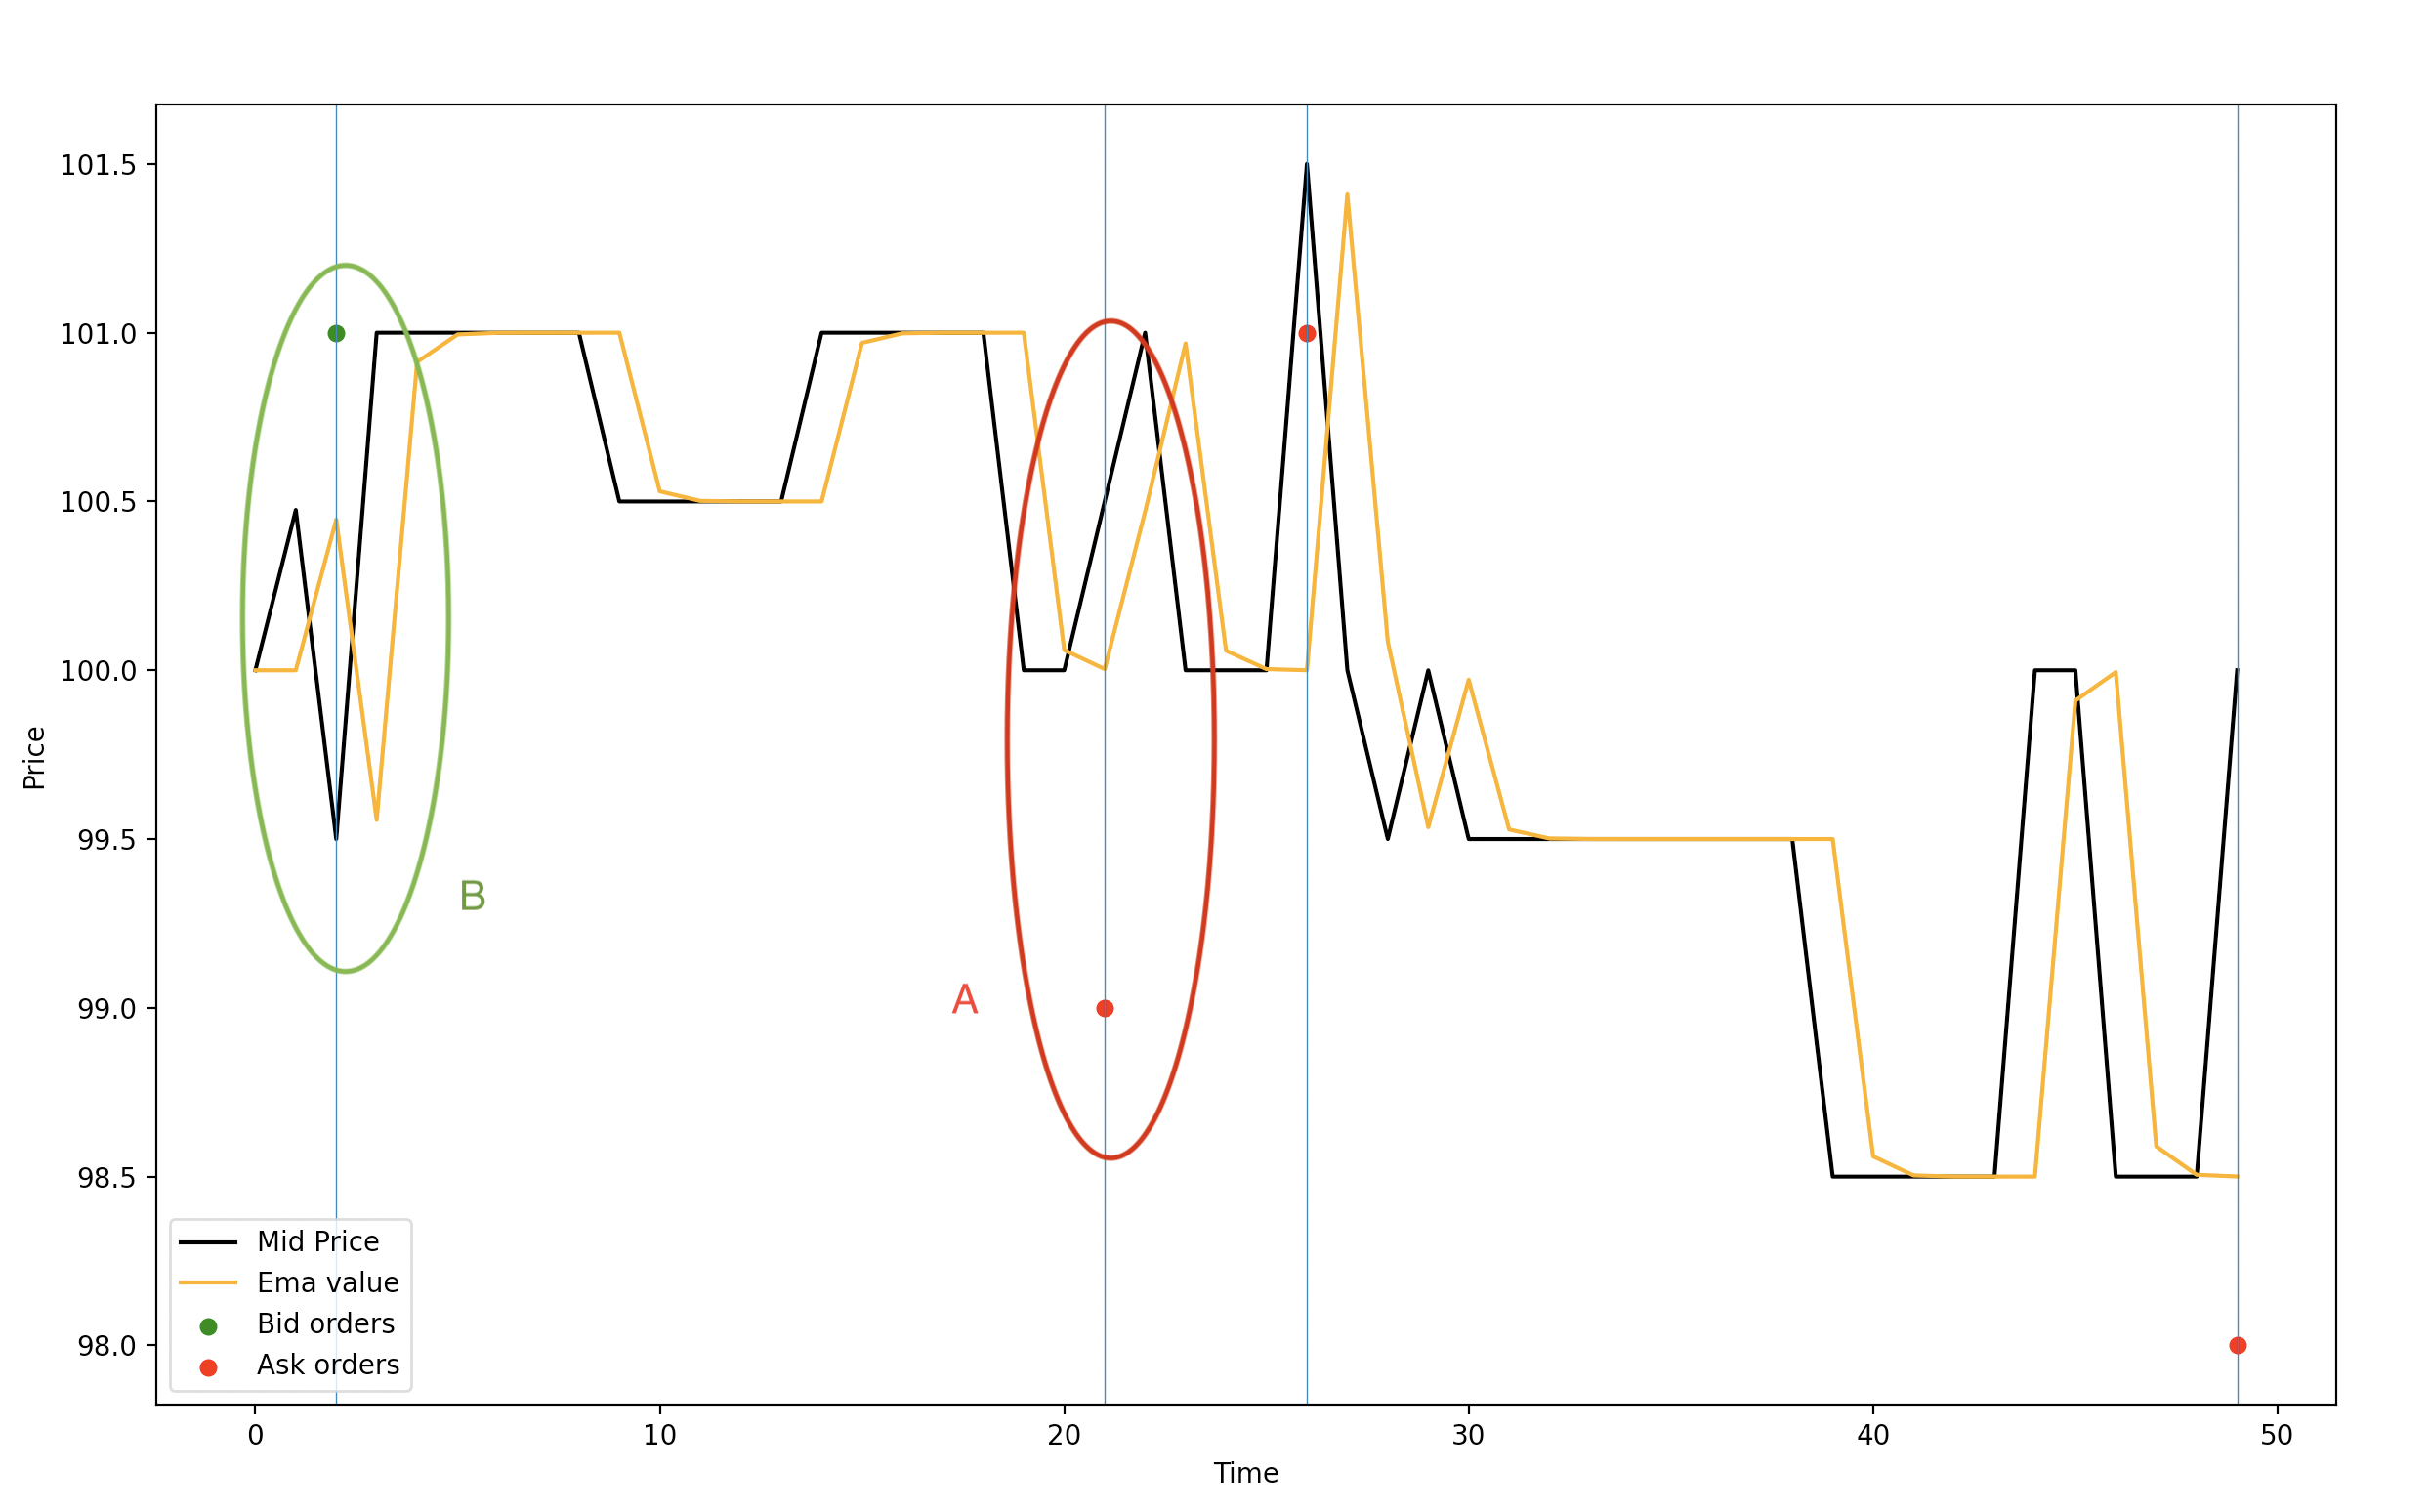
\includegraphics[ height=8cm]{Dissertation/images/mcg_indv/MEAN_R/sample.png}
\caption{Simple Agents and Mean reversion trader Experiment} 
\end{figure} 
\FloatBarrier

The behaviour of the Mean reversion trader can be illustrated by the three points depicted in Figure 5.3. 
\begin{itemize}
  \item \textbf{B} : This depict a point where the $ema_{t}$ value is above the mid price. This means that the mean reversion trader will submit a bid order because it believes that the price will eventually go up back to the moving average. The green dot at the top of the point illustrates a bid order submitted at the best bid price. 
  \item \textbf{B} : This depict a point where the $ema_{t}$ value is below the mid price. This means that the mean reversion trader will submit an ask order because it believes that the price will eventually go down or return to the moving average. The red dot at the peak of the point illustrates an ask order submitted at the best ask price. 
\end{itemize}

However, this also represents a problem. The $ema_{t}$ line is not similar to what is commonly see in other literature. I've decided to change the ema equation. 

\begin{equation}
ema_t = (p_{t} - ema_{t-1}) * (2 / n + 1) + ema_{t-1} 
\end{equation}
where n = period.

If the McG value of 0.94 is calculated using this equation, then the period would be 1.1, which is the same as taking only the previous value into account. However, with the new equation, the coefficient will be 0.04, which is much less than the value specified in McG paper. 

\begin{figure}[h]
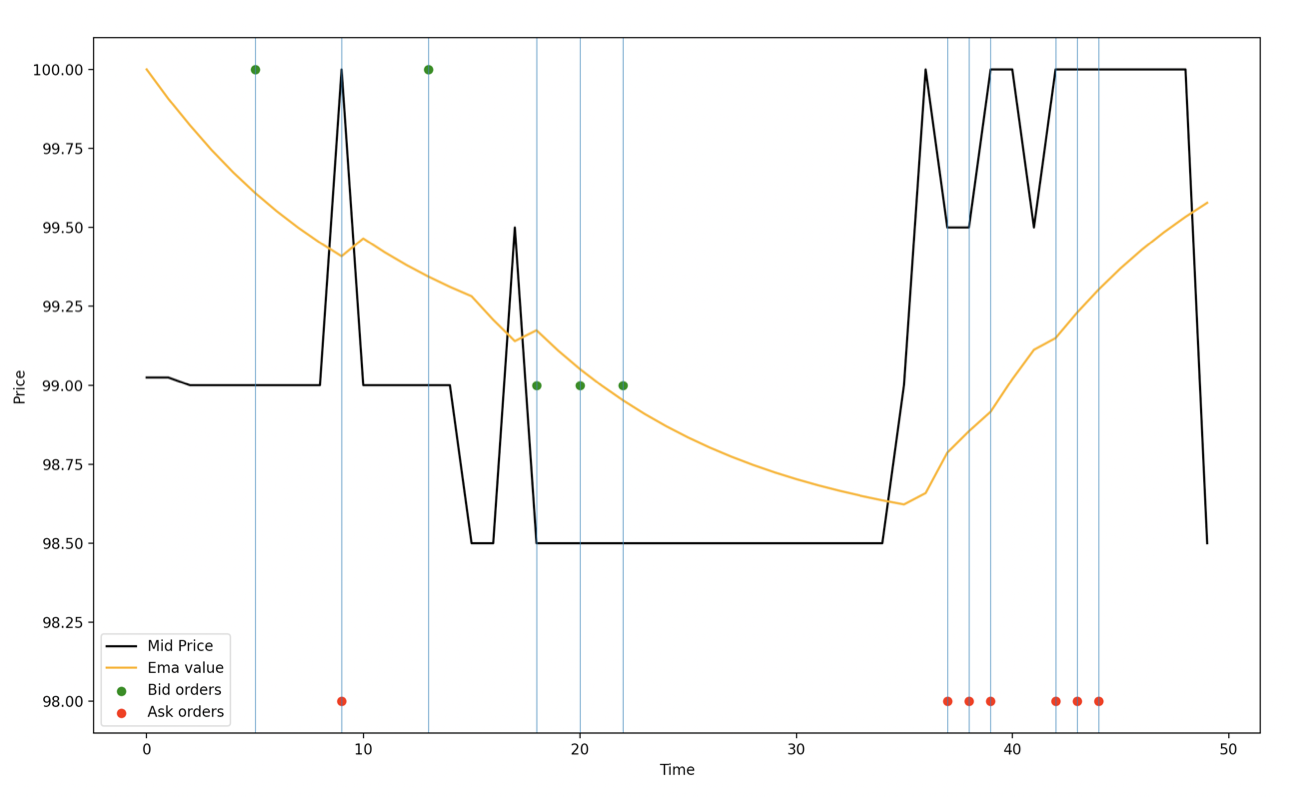
\includegraphics[ height=8cm]{Dissertation/images/mcg_indv/MEAN_R/online.png}
\caption{Simple Agents and Mean reversion trader Experiment} 
\end{figure} 
\FloatBarrier

The figure above illustrates the same experiment with the new $ema_t$ equation. The Mean reversion agent still submits the orders in the same behaviour but the $ema_t$ line is much similar to that of other literature. 

\section{Noise trader} 
The noise trade is also based on Cui and Barbazon \cite{CuiNoise} conference paper. The parameters are very similar except for $xmin_{offspr}$ which changes from 0.05 to 0.005 in the McG implementation. The parameters are given below. 

\begin{table}[h]
\centering
\begin{tabular}{ |m||p{4cm}|} 
\hline
\textbf{Noise Trader Parameters}& \textbf{Value} \\
\hline
\hline
buy or sell & 0.5 \\ 
\hline
Market order probability & $\lambda_{m}$ = 0.03\\ 
\hline
Limit order probability & $\lambda_{l}$ = 0.54\\ 
\hline
Cancel order probability & $\lamda_{c}$ = 0.43\\
\hline 
Market order quantity & $\mu_{mo} = 7 \sigma_{mo} = 0.1 $\\
\hline
Limit Order quantity &  $\mu_{lo} = 8 \sigma_{lo} = 0.7 $\\
\hline
Off-spread relative price & $xmin_{offspr} =0.005$ 
\newline 
$\Beta_{offspr} = 2.72 $\\
\hline
\textbf{Limit order types} & \\
\hline
Crossing limit order & $\lamda_{crs} = 0.003$\\
\hline 
Inside-spread Limit order & $\lamda_{inspr} = 0.098$\\
\hline 
Spread Limit order & $\lamda_{spr} = 0.173$\\
\hline 
Off-spread Limit order & $\lamda_{offspr} = 0.726$\\
\hline
\end{tabular}
\caption{Noise trader parameters taken from \cite{McGroarty}}
\end{table}
\FloatBarrier 

The noise trader is intended to represent other forms of behaviour in the market. By looking at the parameters of the noise trader, it is clear that the noise agent will mostly either submit a limit order or cancel an order. By taking a closer look at the limit order, the agent will mostly submit an Off-spread limit order. According to Cui and Barbazon \cite{CuiNoise}, the Off-spread price of the order is given by the $BestBid - RP_{offspr}$ in a bid order and $BestAsk + RP_{offspr}$ in an ask order. The value $RP_{offspr}$ is given by $xmin_{offspr} * (1-u_0)^{-\frac{1}{\beta - 1}}$. This is equivalent to the price below the Best Bid and above the Best Ask.

By looking the values of the $RP_{offspr}$, one can predict what the range of the price submitted can be. 

\begin{table}[h]
\centering
\begin{tabular}{ |m||p{4cm}|} 
\hline
\textbf{Uniform random value $u_0$}& \textbf{$RP_{offspr}$ Value} \\
\hline
\hline
0 & 0.5\\
\hline 
0.1 & 0.5\\
\hline 
0.2 & 0.4\\
\hline 
0.3 & 0.4\\
\hline 
0.4 & 0.4\\
\hline 
0.5 & 0.3\\
\hline 
0.6 & 0.3\\
\hline 
0.7 & 0.2\\
\hline 
0.8 & 0.2\\
\hline 
0.9 & 0.1\\
\hline 
1.0 & 0.0\\
\hline
\end{tabular}
\caption{Noise trader parameters taken from \cite{McGroarty}}
\end{table}
\FloatBarrier 

The table of values of $RP_{offspr}$ illustrates that the values of the off-spr price should not varied much from the initial price in the beginning. The figure below illustrates that price that the noise trader submits within a market of homogeneous 6 noise agents running with 3000 McG time-period or ten-percent of the whole run-time.The initial price is 100 and the spread is 0.5. 

\begin{figure}[!htbp]
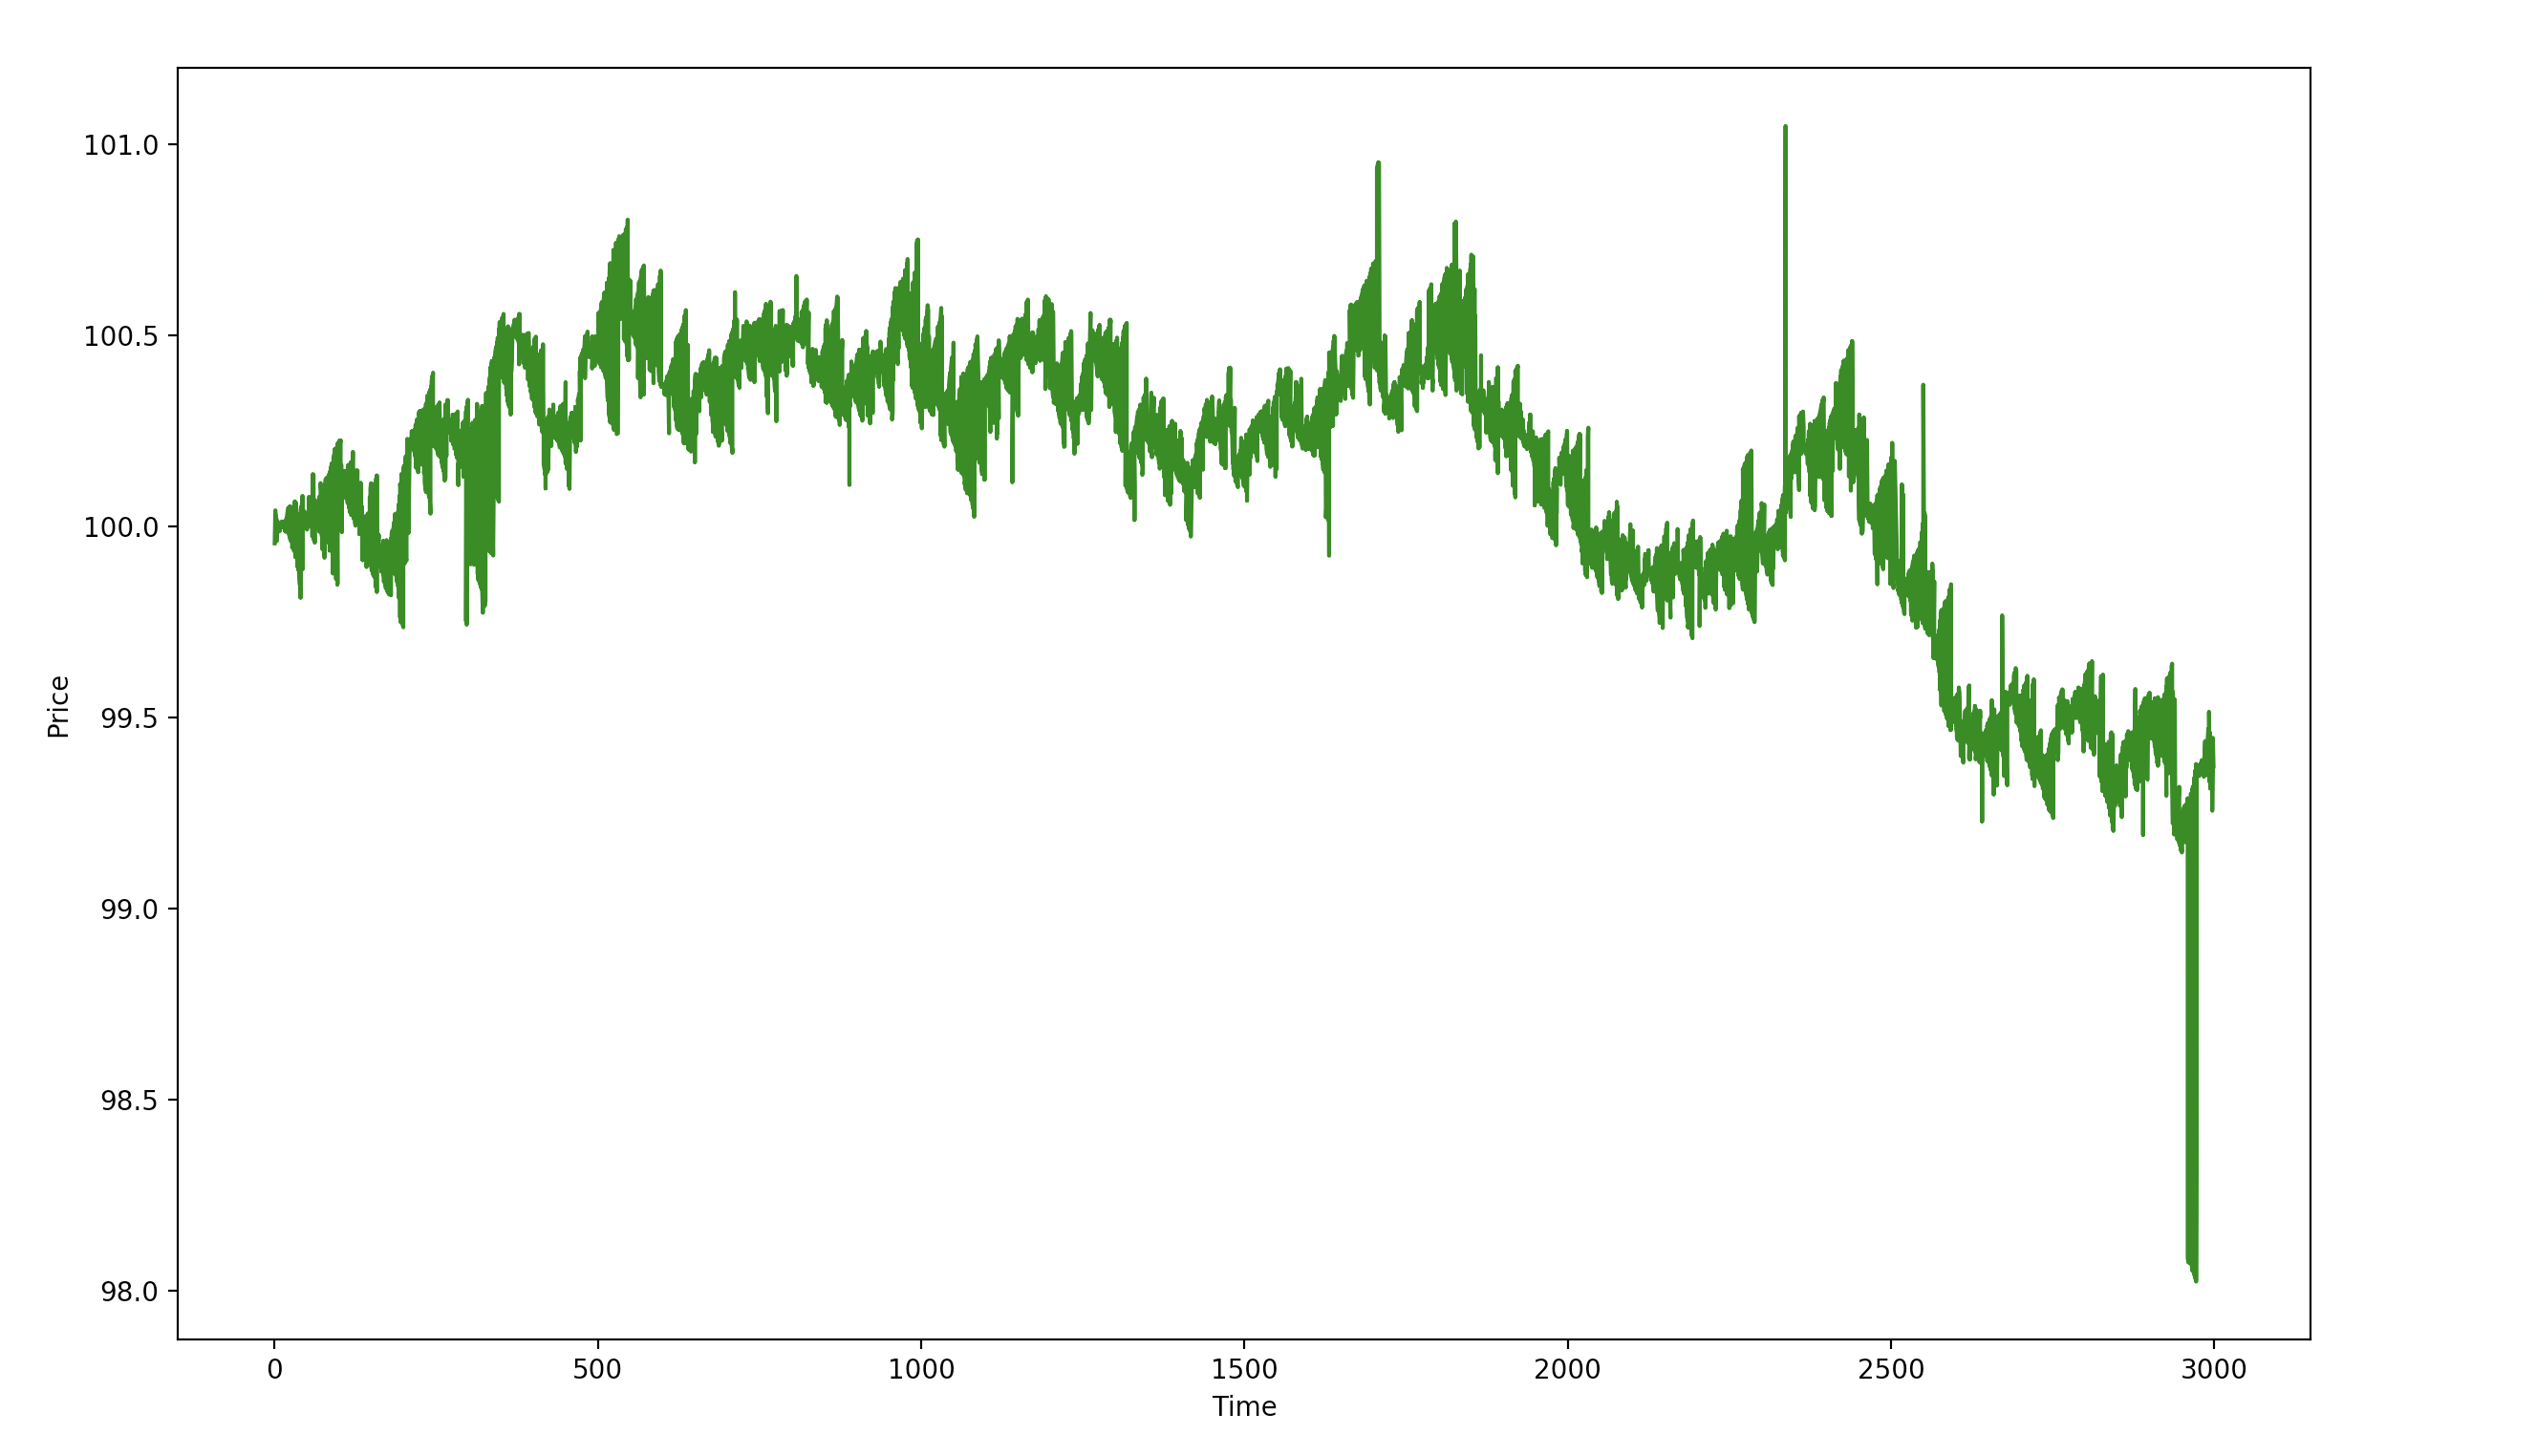
\includegraphics[ height=8cm]{Dissertation/images/mcg_indv/Screenshot 2020-03-20 at 14.33.18.png}
\caption{Noise trader order price} 
\end{figure} 
\FloatBarrier

 
As expected, the price is hugely volatile, due to the random variable of the off-spread price and inside spread limit order. However, the range is still near the initial price and gradually decreases due to the sudden decrease by 0.5 from the off-spr price, which is what can be expected. 

\begin{table}[h]
\centering
\begin{tabular}{ |l||l|l|p{4cm}|} 
\hline
\textbf{Order types} & \textbf{Probability} & \textbf{Value from Experiment} & \textbf{Rough sketch of calculation} \\
\hline
\hline
Ask order & 0.5 & 4877 & $(9284 + 554) / 2 = 4919 \approx 4877$\\ 
\hline
Bid order & 0.5 & 4961 & $(9284 + 554) / 2 = 4919 \approx 4919$\\ 
\hline
\hline
Market order & 0.03 & 554 & $(9284 + 554 + 8162) * 0.03 = 540 \newline \approx 554$\\ 
\hline
\hline
Limit order & 0.54 & 9284 & $(9284 + 554 + 8162) * 0.54 = 9720$  
\newline $\approx 9284 $\\ 
\hline
Crossing Limit Order & 0.003 & 26 & $9284 * 0.003 = 28 \approx 26 $\\ 
\hline
Inside-spread Limit Order & 0.098 & 901 & $9284 * 0.098 = 909 \approx 901 $\\ 
\hline
Spread Limit Order & 0.173 & 1709 & $9284 * 0.173 = 1606 \approx 1709 $\\ 
\hline
Off-spread Limit Order & 0.726 & 6648 & $9284 * 0.726 = 6740 \approx 6648 $\\ 
\hline
\hline
Cancel existing order & 0.43 & 8162 & $(9284 + 554 + 8162) * 0.43 = 7740 \newline \approx 8162 $\\ 
\hline
\end{tabular}
\caption{Noise trader experiment statistics} 
\end{table}
\FloatBarrier 

In most cases, the results line up with the statistics shown as well as the proportion of the orders types submitted.